%%
%% This is file `thesis.tex',
%% generated with the docstrip utility.
%%
%% The original source files were:
%%
%% nudtpaper.dtx  (with options: `thesis')
%% 
%% This is a generated file.
%% 
%% Copyright (C) 2018 by TomHeaven <hanlin_tan@nudt.edu.cn>
%% 
%% This file may be distributed and/or modified under the
%% conditions of the LaTeX Project Public License, either version 1.3a
%% of this license or (at your option) any later version.
%% The latest version of this license is in:
%% 
%% http://www.latex-project.org/lppl.txt
%% 
%% and version 1.3a or later is part of all distributions of LaTeX
%% version 2004/10/01 or later.
%% 
%% To produce the documentation run the original source files ending with `.dtx'
%% through LaTeX.
%% 
%% Thanks LiuBenYuan <liubenyuan@gmail.com> for maintainence.
%% Thanks Xue Ruini <xueruini@gmail.com> for the thuthesis class!
%% Thanks sofoot for the original NUDT paper class!
%% 
%1. 规范硕士导言
% \documentclass[master,ttf]{nudtpaper}
%2. 规范博士导言
% \documentclass[doctor,twoside,ttf]{nudtpaper}
%3. 如果使用是Vista
% \documentclass[master,ttf,vista]{nudtpaper}
%4. 建议使用OTF字体获得较好的页面显示效果
%   OTF字体从网上获得,各个系统名称统一,不用加vista选项
%   如果你下载的是最新的(1201)OTF英文字体,建议修改nudtpaper.cls,使用
%   Times New Roman PS Std
% \documentclass[doctor,twoside,otf]{nudtpaper}
%   另外,新版的论文模板提供了方正字体选项FZ,效果也不错哦
% \documentclass[doctor,twoside,fz]{nudtpaper}
%5. 如果想生成盲评,传递anon即可,仍需修改个人成果部分
% \documentclass[master,otf,anon]{nudtpaper}
%
\documentclass[doctor,ttf,anon]{nudtpaper}
%\usepackage{lmodern} % 这个包导致英文字体与Word的渲染效果不一致,故去掉
\usepackage{mynudt}
\usepackage{multirow,array}

\classification{TP391}
\serialno{1605xxxx}
\confidentiality{公开}
\UDC{681}
\title{基于元学习的小样本空天目标识别\\技术研究}
\displaytitle{基于元学习的小样本空天目标识别技术研究}
\author{陈凌峰}
\zhdate{\zhtoday}
\entitle{Joint Demosaicing and Denoising of Bayer Images}
\enauthor{Tom Heaven}
\endate{\entoday}
\subject{微电子科学与工程}
\ensubject{Control Science and Engineering}
\researchfield{雷达目标识别}
\supervisor{户XX\quad{}副教授}
\cosupervisor{}  % 协助指导教师,没有就空着
\ensupervisor{Prof. XX Hu}
\encosupervisor{} % 协助指导教师英文,没有就空着
\papertype{工学}
\enpapertype{Engineering}
% 加入makenomenclature命令可用nomencl制作符号列表。

\begin{document}
	\graphicspath{{figures/}}
	% 制作封面,生成目录,插入摘要,插入符号列表 \\
	% 默认符号列表使用denotation.tex,如果要使用nomencl \\
	% 需要注释掉denotation,并取消下面两个命令的注释。 \\
	% cleardoublepage% \\
	% printnomenclature% \\
	\maketitle
	\frontmatter
	\tableofcontents
	\listoftables
	\listoffigures
	
	\midmatter
	\begin{cabstract}
国防科技大学是一所直属中央军委的综合性大学。1984年,学校经国务院、中央军委和教育部批准首批成立研究生院,%
肩负着为全军培养高级科学和工程技术人才与指挥人才,培训高级领导干部,从事先进武器装备和国防关键技术研究的重要任务。%
国防科技大学是全国重点大学,也是全国首批进入国家“211工程” 建设并获中央专项经费支持的全国重点院校之一。%
学校前身是1953年创建于哈尔滨的中国人民解放军军事工程学院,简称“哈军工”。
\end{cabstract}
\ckeywords{国防科技大学; 211; 哈军工}

\begin{eabstract}
National University of Defense Technology is a comprehensive national key university based in Changsha, %
Hunan Province, China. It is under the dual supervision of the Ministry of National Defense %
and the Ministry of Education, designated for Project 211 and Project 985, %
the two national plans for facilitating the development of Chinese higher education. %

NUDT was originally founded in 1953 as the Military Academy of Engineering in Harbin of Heilongjiang Province. %
In 1970 the Academy of Engineering moved southwards to Changsha and was renamed Changsha Institute of Technology.%
 The Institute changed its name to National University of Defense Technology in 1978.

\end{eabstract}
\ekeywords{NUDT; MND; ME}


	\chapter*{符号使用说明}
% 可以根据需要在chapter后加星星/去掉星星

\begin{denotation}

\item[HRRP] 高分辨率距离像 (High-Resolution Range Profile)
\item[RATR] 雷达自动目标识别 (Radar Automatic Target Recognition)
\item[FSL] 小样本学习 (Few-Shot Learning)
\item[MAML] 模型无关元学习 (Model-Agnostic Meta-Learning)
\item[GNN] 图神经网络 (Graph Neural Network)
\item[VLM] 视觉语言模型 (Visual Language Model)
\item[SNR] 信噪比 (Signal-to-Noise Ratio)
\item[GAF] 格拉姆角场 (Gramian Angular Field)
\item[CNN] 卷积神经网络 (Convolutional Neural Network)
\item[CLIP] 对比语言-图像预训练 (Contrastive Language-Image Pre-training)
\item[$\mathcal{T}$] 元学习任务 (Meta-learning Task)
\item[$\mathcal{S}$] 支持集 (Support Set)
\item[$\mathcal{Q}$] 查询集 (Query Set)
\item[$N$] 任务类别数 (N-way)
\item[$K$] 每类样本数 (K-shot)
\item[$\Theta, \Phi$] 模型参数 (Model Parameters)
\item[$\mathcal{L}$] 损失函数 (Loss Function)
\item[$\mathbf{A}$] 邻接矩阵 (Adjacency Matrix)
\item[$\mathbf{H}$] 节点特征矩阵 (Node Feature Matrix)
\item[$z_V, z_T$] 视觉/语义特征 (Visual/Semantic Features)
\item[$p_c$] 类别原型 (Class Prototype)
\item[$\mathbf{p}$] HRRP样本向量 (HRRP sample vector)
\item[$\theta, \phi$] 目标姿态角 (Target aspect angles)
\item[$f_c$] 雷达载频 (Radar carrier frequency)
\item[$B$] 信号带宽 (Signal bandwidth)
\item[$\Delta R$] 距离分辨率 (Range resolution)

\end{denotation}
	
	%书写正文,可以根据需要增添章节; 正文还包括致谢,参考文献与成果
	\mainmatter
	\renewcommand\UrlFont{\timesnr}
	\makeatletter
	\newcounter{blankpages}
	\def\cleardoublepage{%
		\clearpage
		\if@twoside
		\ifodd\c@page
		\else
		\hbox{}\newpage\stepcounter{blankpages}%
		\thispagestyle{empty}%
		\if@twocolumn\hbox{}\newpage\fi
		\fi
		\fi
	}
	\newcommand{\@romannoblank}[1]{%
		\@roman{\numexpr#1-\value{blankpages}\relax}%
	}
	\makeatother
	
	\chapter{绪论}

\section{研究背景与意义}

在全球战略格局深刻调整与新一轮科技革命加速演进的背景下,空天领域已成为衡量国家综合实力和维护国家安全的核心战略疆域~\cite{X}。确保我国在空天领域的安全、自主与战略主动,对于实现国家现代化发展目标具有不可替代的基础性作用。空天技术的飞速发展催生了数量庞大、性能先进、行为模式多样的新型空天目标,如高超声速飞行器~\cite{X}、大规模低轨卫星星座~\cite{X}、隐身作战平台及无人机集群~\cite{X}等。这些目标普遍具有的高动态、低可探测、智能化和网络化特征,对现有国家防空预警、空间态势感知乃至整体空天防御体系的有效性构成了前所未有的挑战,显著增加了对其进行可靠探测、跟踪、识别与处置的复杂性和难度~\cite{X}。

面对此严峻态势,发展先进的空天目标识别能力,实现对各类目标的及时发现、稳定跟踪、精确分类与可靠评估,已成为构筑坚实国家空天安全屏障、支撑高效军事行动与明智战略决策的核心要素~\cite{X}。精确的目标识别是有效拦截、精确打击、威胁评估、意图判断等一系列后续行动的基础。缺乏准确的目标属性信息,将导致空天态势认知模糊,指挥控制效能下降,信息优势难以确立。尤其是在现代战争所特有的复杂电磁环境和高强度对抗条件下,能否快速、准确地判明目标的具体类型、型号乃至身份,直接关系到作战资源的优化配置、战场迷雾的有效驱散以及战略误判风险的管控~\cite{X}。近期如俄乌冲突与巴以冲突等局部战争的实践,更是直观地展示了在无人平台、精确制导弹药和先进传感器广泛应用的现代战场上,空天目标精确识别能力对于实时战场态势生成、作战效果评估乃至冲突走向的关键性影响。准确识别敌方高价值节点(如指挥控制中心、关键传感器)和主要威胁(如来袭导弹、攻击无人机),已成为夺取战场主动权、提升作战效能的核心环节。因此,先进的目标识别技术已成为现代军事体系不可或缺的关键技术支撑。

鉴于空天目标识别的极端重要性,世界主要国家均将其置于国防科技发展的优先地位~\cite{X}。美国凭借其强大的研发体系,持续投入于先进传感器、智能信息处理及网络化监视系统的建设,特别是在人工智能(尤其是深度学习)应用于目标识别领域保持领先~\cite{X}。欧洲国家通过多边合作,在高性能雷达、卫星侦察和多源融合技术方面不断取得进展~\cite{X}。俄罗斯等国则在应对特定威胁(如高超声速目标)和复杂对抗环境下的识别技术上展现其特色。各国研究的共同焦点在于如何克服目标信号微弱、动态性强、背景扰动复杂、目标类型多样及智能化对抗等技术难题,并积极利用人工智能、大数据、多传感器协同等新兴技术,实现对空天目标的{全域、全时、全谱}精确感知与深度认知~\cite{X}。

对于我国而言,维护国家统一、保障领土完整、拓展海外利益以及推进海洋强国、航天强国等战略目标的实现,均对空天态势感知与目标识别能力提出了极高要求~\cite{X}。我国面临的空天安全环境复杂,潜在威胁来源多样,涵盖从高性能隐身平台、战略武器,到临近空间与轨道空间的新型飞行器、各类卫星,再到低小慢无人机等不同维度~\cite{X}。若无法对这些潜在威胁进行有效识别,国家空天预警防御体系将存在关键短板,直接威胁国家安全。同时,随着国家利益的全球化和自身空天活动的日益频繁(如空间站运营、北斗全球服务、密集卫星部署、繁忙民航交通等),保障海外利益和自身空天资产安全的需求也日益凸显。准确识别空间碎片、非合作接近目标或攻击威胁,是维护我国空天基础设施稳定运行、支撑经济社会发展的重要保障~\cite{X}。因此,发展自主可控、国际先进的空天目标自动识别技术体系,全面提升精确识别与深度理解能力,不仅是应对现实安全挑战的迫切需要,更是支撑国家重大战略、提升综合国力的基础工程。攻克非合作目标精确识别等技术难题,是我国国防科技领域必须抢占的战略制高点。本研究正是立足于此重大战略需求,聚焦于空天目标识别技术链中的核心挑战,旨在通过深入研究为提升我国在该领域的自主创新能力提供理论与技术支撑。

在空天目标探测识别的多种技术手段中,雷达系统凭借其独特的物理原理和工程优势,长期以来在空天感知体系中扮演着核心角色,并预计在未来仍将保持其骨干地位~\cite{X}。作为主动探测设备,雷达的核心优势首先体现在其{全天候、全天时}的工作能力,电磁波传播基本不受光照、云、雾、雨、雪等气象条件限制,确保了探测系统的连续性和可靠性,这与依赖环境条件的光学、红外等被动手段形成鲜明对比~\cite{X}。其次,雷达通常具备{作用距离远、覆盖范围广}的特点,能够对广阔空域或空间进行有效搜索与监视,为后续处理提供必要的预警时间~\cite{X}。更为关键的是,雷达不仅能精确测量目标的距离、方位、速度等运动学参数,还能通过精细分析回波信号的{幅度、相位、频率、极化}等特征,反演目标的{物理属性}(如尺寸、形状、结构、材质)和{精细运动状态}(如姿态、微动),为非合作目标的精确识别提供了不可或缺的信息来源~\cite{X}。

现代雷达技术的进步,特别是宽带信号处理和高分辨率成像技术的发展,极大地提升了雷达获取目标细节信息的能力~\cite{X}。宽带信号的应用提高了距离分辨率,能够分辨目标沿雷达视线(Line of Sight,LOS)的散射中心分布,形成{高分辨率距离像(High Resolution Range Profile,HRRP)}~\cite{X}。HRRP蕴含了目标一维结构信息,是雷达自动目标识别(Radar Automatic Target Recognition,RATR)研究中最常用的一类特征~\cite{X}。同时,{合成孔径雷达(Synthetic Aperture Radar,SAR)}~\cite{X}与{逆合成孔径雷达(Inverse-SAR,ISAR)}~\cite{X}等成像技术能够生成目标的二维甚至三维高分辨率图像,直观展示其几何形态和散射点布局,为识别提供了更丰富的信息。这些高分辨率技术的发展,为RATR技术奠定了基础,使其成为提升空天态势感知智能化水平的关键途径~\cite{X}。回顾其发展历程,RATR技术大致经历了从早期的{模板匹配}~\cite{X},到中期的{特征工程与浅层分类器}~\cite{X},再到近十余年来由{深度学习}驱动的新阶段~\cite{X}。深度神经网络凭借其强大的{自动特征学习}和{非线性建模}能力,实现了“端到端”的识别,在数据充足时显著超越了传统方法,成为当前研究的主流范式。国际主要研究机构均在积极探索深度学习在RATR各方向(如SAR及ISAR图像分类、HRRP序列识别、微多普勒分析)的应用~\cite{X}。

然而,尽管深度学习带来了巨大进步,但将其成功应用于实际复杂环境的RATR仍面临源于物理限制和应用场景复杂性的严峻挑战~\cite{X}。{一方面,雷达目标特征的内在复杂性与对观测条件的极端敏感性依然是核心难题~\cite{X}。} 电磁散射过程受多重因素耦合影响,导致雷达特征(特别是HRRP)对目标姿态角变化极为敏感(即{“姿态敏感性”}),微小变动即可引起特征剧烈畸变,严重影响识别稳定性~\cite{X}。SAR等二维像同样存在角度依赖性,且成像质量受运动状态影响~\cite{X}。目标微动引入的微多普勒效应进一步增加了信号的复杂度。因此,从复杂、时变、敏感的雷达信号中提取稳定且具判别力的特征表示,始终是RATR领域的核心科学问题。{另一方面,真实电磁环境中的噪声、杂波是制约RATR实际性能的关键障碍~\cite{X}。} 雷达信号不可避免地混杂背景杂波(地杂波、海杂波、气象杂波),这些{噪声和杂波}严重降低了信号质量,污染甚至淹没目标特征,对后续处理造成极大困难。如何在低信噪比条件下实现{稳健识别},是衡量RATR系统实用价值的关键指标。

{此外,当前最为突出的瓶颈是高质量、大规模、标注完备的训练数据普遍严重匮乏,即“小样本问题”~\cite{X}。} 深度学习的性能高度依赖大数据训练,但在RATR领域,获取此类数据的成本高昂、限制众多(实测获取难)、目标类型动态变化(数据库难完备)、状态多样性导致样本需求巨大、数据标注困难且昂贵、仿真数据与实测数据间存在显著“域差异”(Domain Gap)等因素共同导致了训练样本的稀缺~\cite{X}。这种数据稀缺性与深度模型的数据需求之间的矛盾,构成了当前RATR发展的核心困境。在小样本条件下,深度模型极易{过拟合},导致{泛化能力}严重不足。因此,研究如何在有限标注样本下实现高效、可靠的识别,提升模型的泛化性和对新目标的快速适应能力,已成为推动RATR技术走向实用化的关键突破口。

{最后,现有方法在利用目标语义信息方面尚显不足。} 多数方法依赖底层物理特征,而目标本身蕴含的{语义信息}(如类别、功能、型号、威胁等级等)对于区分相似目标、理解意图、辅助决策具有重要价值~\cite{X}。在小样本或低分辨条件下,对于物理特征目标区分度不足的情况,融合语义信息有望提升识别精度和可靠性。然而,如何有效表示、融合跨模态的物理特征与语义信息,并将其整合到学习与推理过程中,仍是待深入探索的研究方向。

面对上述局限与挑战,RATR技术呈现出以下主要发展趋势:一是持续追求更高质量的特征信息获取(更高分辨率~\cite{X}、更精细特征~\cite{X});二是发展更智能、适应性更强的识别模型(深度学习与雷达特性深度融合,如时空建模~\cite{X}、自监督~\cite{X}、持续学习~\cite{X});三是显著提升模型在复杂环境下的鲁棒性(抗噪抗扰设计~\cite{X},物理知识引导的机器学习~\cite{X});四是{集中力量攻克小样本学习难题},其中,以{元学习(Meta-Learning)}为代表的“学会学习”范式,因其在快速适应新任务、提高样本效率方面的潜力而备受关注~\cite{X},是本论文的核心研究方法;五是积极探索多源信息融合与协同识别~\cite{X};六是日益关注模型的可解释性、可信赖性与安全性~\cite{X}。

综上所述,RATR技术的发展机遇与挑战并存。以深度学习为代表的AI技术注入了新活力,但也使其在数据依赖(特别是小样本困境)、环境适应性、特征复杂性等方面面临严峻制约。有效解决小样本学习问题,提升模型在真实复杂环境下的鲁棒性、泛化能力和快速适应能力,是当前RATR领域亟待突破的核心技术瓶颈。本研究正是围绕此瓶颈,以元学习为主要理论框架,深入研究其在解决小样本雷达HRRP目标识别问题中的应用潜力,特别是在应对噪声扰动、角度敏感性和语义信息利用等具体技术难点方面,提出针对性的创新方法,旨在为提升我国空天目标精确识别技术水平提供理论与技术储备。

\section{空天目标RATR技术研究现状}
前文深入探讨了空天目标精确识别的战略紧迫性,并分析了雷达作为核心传感手段的优势、局限及发展趋势,特别指出了“小样本问题”是制约当前先进识别算法性能的关键瓶颈。在此基础上,本节将进一步聚焦于RATR领域如何应对数据稀缺性的挑战。我们将首先回顾传统RATR方法为何在处理复杂性和小样本问题上存在固有的局限性;接着,阐述深度学习方法如何作为一种更强大的范式被引入RATR领域,并分析其在带来性能提升的同时,如何使得小样本问题变得更为突出和关键;最后,在此背景下,系统梳理当前专门针对小样本RATR的研究现状、主要技术途径及其面临的持续挑战。

在深度学习技术广泛应用之前,RATR的研究主要沿着两条技术路径发展:基于模板匹配~\cite{X}和基于特征工程与浅层分类器~\cite{X}。模板匹配方法通过将待测目标特征与预建模板库进行比对来识别,原理直观,但在面对目标多样性、姿态剧变以及模板库难以完备的现实时,尤其是在可用样本稀少、无法构建代表性模板库的小样本条件下,其性能和鲁棒性显著不足~\cite{X}。为了克服这些限制,研究转向了特征工程路线,即人工设计对特定变化(如姿态、噪声)相对不敏感的稳健特征,再结合SVM、KNN等浅层分类器进行判决~\cite{X}。这种方法通过特征提取实现了信息抽象,提升了一定的灵活性和鲁棒性。然而,其成功严重依赖于特征设计的质量,并且需要深厚领域知识、耗时费力且泛化能力有限。特别是在小样本条件下,缺乏足够数据指导特征设计与验证,难以获得真正具有普适判别力的特征~\cite{X}。同时,浅层分类器有限的模型容量也难以充分捕捉雷达数据内在的高度非线性复杂关系,限制了识别性能的上限~\cite{X}。因此,尽管传统方法为RATR奠定了基础,但它们在特征表示能力、模型泛化性、自动化程度以及应对小样本挑战的能力上均存在明显瓶颈,难以满足现代空天目标识别任务对高精度、高鲁棒性、高适应性的需求~\cite{X}。

{传统方法的上述局限性,特别是其在特征表示学习上的不足和对人工经验的过度依赖,自然而然地推动了研究界寻求更强大的数据驱动模型~\cite{X}。深度学习凭借其从大规模数据中自动学习层次化特征表示的卓越能力,在计算机视觉等领域取得革命性成功后,也被迅速引入RATR领域~\cite{X}。以卷积神经网络(Convolutional Neural Network,CNN)~\cite{X}、循环神经网络(Recurrent Neural Network,RNN)~\cite{X}及其变种~\cite{X}、长短时记忆网络(Long-Short Term Memory,LSTM)~\cite{X}、图神经网络(Graph Neural Network, GNN)~\cite{X}以及近年备受关注的Transformer架构~\cite{X}为代表的深度模型,能够直接处理雷达二维像(SAR或ISAR)或序列数据(HRRP),实现了“端到端”的识别流程,在数据相对充分的条件下,展现出超越传统方法的性能潜力~\cite{X},标志着RATR技术进入了一个新的发展阶段。

然而,深度学习的强大性能与其大规模标注数据驱动的特性是一体两面~\cite{X}。虽然RATR领域的数据稀缺问题由来已久,但在深度学习范式下,这个问题变得尤为尖锐和关键。深度模型通常包含数百万甚至更多的参数,需要海量的、多样性的标注样本进行有效训练才能避免过拟合,学习到具有良好泛化能力的特征表示~\cite{X}。但在RATR领域,如前文(1.1.2节)所述,获取大规模、高质量、标注完备的实测数据面临着成本、限制、目标多样性、状态多变性、标注难度以及仿真数据域差异等多重现实障碍。这种深度模型对数据的强依赖性与雷达数据获取的固有困难之间的矛盾,使得{小样本问题从一个普遍存在的挑战,升级为制约深度学习RATR技术实用化、发挥其全部潜力的核心瓶颈}。直接将标准深度学习模型应用于典型的雷达小样本场景,往往导致模型训练不足、过拟合严重,识别性能远达不到预期。因此,如何在深度学习框架下有效应对数据稀缺性,成为RATR领域亟待解决的关键科学问题,直接催生了针对性的{小样本学习(Few-Shot Learning, FSL)}研究方向~\cite{X}。

% ... (保持 1.1 节和 1.2.1 节内容不变) ...

\section{小样本RATR技术面临的挑战}
% 调整本小节开头,明确先总后分
面对传统方法的局限以及深度学习范式下凸显的小样本瓶颈,FSL已成为推动RATR技术发展的关键研究方向~\cite{X}。FSL旨在使模型具备从极少量标注样本中学习并泛化到新类别或新任务的能力~\cite{X}。近年来,研究者们已将多种源于通用机器学习领域的FSL策略引入小样本RATR研究,并针对雷达数据的特性进行了初步的适应与发展。本小节将首先概述这些主流技术途径在RATR领域的应用现状,然后重点剖析本研究所关注的三个核心挑战及其现有研究的不足之处。

% 概述主流FSL方法在RATR中的应用现状
当前应用于小样本RATR的主流FSL技术途径大致可分为以下几类:

{一是基于数据增广(Data Augmentation)的策略~\cite{X}。} {作为缓解数据不足最直接的手段,数据增广通过变换现有样本或生成新样本来扩充训练集。在RATR领域,除了应用旋转、平移等几何变换(需注意保持物理意义,尤其对HRRP等非图像数据)和添加模拟噪声外,基于深度生成模型(如生成对抗网络GANs、变分自编码器VAEs)的样本合成受到了广泛关注。例如,已有研究利用GANs生成逼真的SAR图像~\cite{X}或HRRP样本~\cite{X},以扩充小样本训练集。西安电子科技大学的研究学者在利用GAN进行雷达数据增广方面进行了深入探索~\cite{X}。然而,数据增广的局限性在于:简单变换难以模拟雷达数据(尤其是HRRP)对姿态等因素的复杂、非线性变化;生成模型的训练本身也需要一定数据基础,且生成样本的质量(逼真度、多样性)和与真实数据分布的一致性难以完全保证,尤其对于结构复杂、细节丰富的雷达特征,GANs可能面临模式坍塌等问题~\cite{X};更重要的是,增广数据并未带来关于新类别目标的本质信息,对于提升模型对全新类别的泛化能力帮助有限,其主要作用在于提升模型在已有类别上的鲁棒性和减少过拟合~\cite{X}。}

{二是基于迁移学习(Transfer Learning)与领域自适应(Domain Adaptation)的策略~\cite{X}。} {迁移学习试图将在数据丰富的源域(如大规模仿真数据集、相关实测数据集)上学到的知识(如预训练模型参数)迁移至数据稀缺的目标域。常见的做法是在源域预训练深度模型,然后在目标小样本数据集上进行微调(Fine-tuning)。这种方法能够利用源域的通用特征表示,加速学习并可能提升小样本性能。例如,研究人员尝试利用仿真数据预训练的模型迁移到实测数据识别任务中~\cite{X}。然而,其有效性高度依赖于源域与目标域的相关性。雷达应用中常见的显著“域偏移”(Domain Shift),如仿真与实测之间、不同雷达参数或环境条件之间,会严重限制迁移效果,甚至导致负迁移~\cite{X}。领域自适应技术致力于显式地减小域间分布差异,例如通过对齐特征分布~\cite{X}或利用对抗学习进行域混淆~\cite{X},以提升模型跨域泛化能力。国防科技大学、电子科技大学等单位在雷达信号处理的迁移学习和领域自适应方面均有深入的研究积累~\cite{X}。尽管这些方法在一定程度上缓解了小样本问题,但它们通常假设目标域仍有一定量(可能未标注)的数据可供适应,对于仅有极少量标注样本(如one-shot)的极端小样本场景或需要快速识别在源域中完全未出现过的新类别的情况,其能力仍然受限~\cite{X}。}

{三是基于元学习(Meta-Learning)的策略,其中亦包含度量学习的思想~\cite{X,X}。} {元学习,或称“学会学习”,被认为是解决小样本问题的更根本性范式。它旨在让模型掌握一种通用的学习策略或获得一个良好的初始状态(元知识),使其能在仅有少量标注样本的新任务上快速适应并有效泛化~\cite{X}。元学习通常采用“任务式”训练框架(元训练),通过优化模型在大量模拟小样本任务上的性能来学习元知识。根据学习元知识的方式,主要可分为:
(1) \emph{基于优化的元学习}:如模型无关元学习(Model-Agnostic Meta-Learning,MAML)~\cite{X}及其变种,目标是学习一个对新任务数据极其敏感、只需少量梯度更新即可快速适应的模型初始化参数。已有研究初步将MAML应用于小样本SAR图像分类~\cite{X}。
(2) \emph{基于度量的元学习}:这类方法的核心思想是学习一个通用的嵌入空间或相似度度量函数,使得在该空间中,同类样本紧密聚集,异类样本相互分离。这使得模型能够基于与少量支持集样本的距离或关系来进行预测。原型网络(Prototypical Networks,ProtoNet)~\cite{X}、匹配网络(Matching Networks,MN)~\cite{X}、关系网络(Relation Networks,RelationNet)~\cite{X}等是其中的代表。这些方法因其简洁有效和天然的小样本适应性而备受关注。例如,原型网络通过计算支持集样本在嵌入空间中的类别原型(均值),然后将查询样本归类到最近的原型,已被尝试应用于小样本HRRP识别~\cite{X}和SAR图像识别~\cite{X}。复旦大学等高校在度量学习理论与应用方面有较多研究~\cite{X}。将度量学习视为元学习的一种重要实现途径(学习通用的度量函数作为元知识)是当前的一个普遍观点。
元学习提供了一个系统性的解决小样本问题的框架,其“学会学习”的思想与RATR需要快速适应新目标、新环境的需求高度契合,展现出巨大的应用潜力。}

{挑战一:低信噪比与复杂噪声扰动下的鲁棒识别。}
雷达信号在传播和接收过程中极易受到各种噪声(热噪声、散粒噪声等)、杂波(地、海、气象杂波)的影响,导致目标信号信噪比(SNR)或信杂比(SCR)显著降低~\cite{X}。在小样本条件下,模型本就难以从有限数据中学习到目标的本质特征,噪声的存在进一步模糊了目标信息,引入了虚假特征,显著加剧了特征提取的困难和模型过拟合的风险,导致识别性能急剧恶化。虽然传统方法中有基于统计特性或信号子空间的抗噪声特征设计~\cite{X},深度学习中也有一些研究关注于设计鲁棒网络结构(如引入残差连接~\cite{X}、注意力机制~\cite{X})或采用去噪自编码器等进行预处理~\cite{X},但这些方法往往存在局限:它们通常假设噪声模型已知或相对简单(如高斯白噪声),或者需要足够的数据来学习噪声的统计特性或训练去噪模型。然而,雷达面临的真实噪声往往是复杂、非平稳、甚至未知的,其强度和类型可能随时间、空间动态变化。
现有的通用FSL方法,包括数据增广(简单添加噪声难以模拟真实复杂噪声)、迁移学习(源域可能无噪声或噪声类型不同)、以及元学习及度量学习,大多在相对干净的数据集上进行验证,普遍缺乏针对雷达领域常见的、强度未知或变化、类型复杂的噪声扰动环境进行鲁棒性设计的内禀考量~\cite{X}。例如,标准的元学习任务构建通常不显式模拟噪声水平的变化,学习到的快速适应能力可能对噪声变化不鲁棒;度量学习所学习的嵌入空间可能对噪声扰动非常敏感,导致同类样本在噪声下距离变大,异类样本距离变小。因此,如何在{样本极其有限}的情况下,使模型具备对{未知或变化的噪声}的自适应鲁棒识别能力,是一个亟待解决的关键难题。目前,专门针对{小样本RATR的噪声鲁棒性}研究相对不足,缺乏能够有效应对未知复杂噪声环境的系统性解决方案~\cite{X}。北京理工大学在复杂电磁环境下雷达信号处理方面有较多积累~\cite{X},但将其与小样本学习特别是元学习深度结合的研究尚待深入。

{挑战二:雷达特征(尤其是 HRRP)的角度敏感性。}
雷达回波特性,特别是HRRP,对目标的观测姿态角(方位角、俯仰角)表现出极端敏感性~\cite{X}。这是由雷达散射的物理机制决定的:HRRP是目标散射中心沿雷达视线的一维投影,姿态角的微小变化会导致视线方向的改变,从而引起散射中心投影位置、遮挡关系以及相对强度的剧烈、非线性变化。这种现象使得同一目标在不同角度下的HRRP样本形态可能差异巨大,甚至超过不同目标之间的差异,严重违反了许多机器学习算法(包括FSL)关于“类内紧凑、类间分离”的基本假设~\cite{X}。这一物理瓶颈是RATR,尤其是基于HRRP识别的固有核心挑战。传统方法尝试通过设计角度不敏感特征(如基于旋转不变量的特征)~\cite{X}或建立覆盖宽角度范围的多姿态模板库~\cite{X}来应对,但前者往往以牺牲大量判别信息为代价,导致识别性能下降;后者则面临模板库构建成本高昂、存储量巨大、匹配效率低以及对未覆盖角度泛化能力差等问题。
深度学习方法,例如使用RNN~\cite{X}或LSTM~\cite{X}处理HRRP序列以捕捉角度变化的时序依赖性,或者设计特定的CNN结构(如角度分离网络)~\cite{X},试图学习角度不变表示或显式建模角度变化规律。然而,在小样本条件下,模型难以从有限的、可能角度覆盖不连续的样本中充分学习到这种复杂的、高度非线性的角度依赖关系,导致跨角度泛化能力差,即在训练时未见过或样本稀少的角度范围上识别性能急剧下降~\cite{X}。现有的通用FSL方法,无论是基于优化还是基于度量,通常假设任务内或类别内的样本具有一定的内在相似性。雷达目标的强角度敏感性恰恰打破了这一假设,使得直接应用这些方法效果受限。虽然已有少量工作尝试将FSL应用于跨角度雷达目标识别~\cite{X},例如南京航空航天大学的研究人员可能探索过相关问题~\cite{X},但这些研究可能未能充分挖掘和利用样本间的角度关联信息(如角度连续性、对称性等物理先验),或者在角度跨度较大、样本极其稀疏的极端小样本场景下性能下降仍然显著。因此,如何在{小样本约束}下,有效克服HRRP等雷达特征的{强角度敏感性},实现对{宽角度范围或未知角度}目标的可靠识别,是小样本RATR领域亟待攻克的另一个核心技术挑战。

{挑战三:小样本下特征判别性不足与语义信息利用匮乏。}
当每类目标的训练样本极少时(例如one-shot或few-shot),模型仅能接触到目标极其有限的观测实例。此时,单纯依赖从雷达物理信号(如HRRP的幅度、相位,SAR或ISAR图像的像素强度)中通过深度网络学习到的底层特征表示,可能不足以有效地区分那些结构相似、雷达散射特性接近的不同目标类别~\cite{X}。这种由于样本稀疏导致的{特征判别性不足}问题,在高相似度目标混杂的识别场景中尤为突出。在这种情况下,目标的{语义信息},即关于目标的高层抽象知识,如其所属的功能类别(例如,战斗机、轰炸机、预警机、运输机)、具体型号家族、甚至依据先验情报判断的威胁等级等,能够提供独立于物理特征的重要补充判别线索。例如,两款在HRRP或SAR图像上看起来相似的飞机,可能分属不同的功能类别,具有迥异的作战用途和威胁程度。如果能在识别决策中有效融入这些语义信息,即使物理特征区分度不高,也有望显著提升识别的准确性和可靠性。
在通用计算机视觉领域,已有大量研究探索将语义信息(如类别名称的词嵌入、属性描述、知识图谱关系等)融入FSL框架,例如通过语义引导的度量学习~\cite{X}或利用语义信息生成分类器权重~\cite{X},并取得了显著效果。然而,在RATR领域,系统性地研究如何获取、表示雷达目标特有的语义信息,并将其有效融入小样本学习框架(特别是元学习)的研究尚处于非常初级的阶段。雷达目标的语义属性可能与视觉目标不同,其获取(可能依赖专业情报数据库或专家知识)和形式化表示(如何与数值化的雷达特征融合)面临独特挑战。如何设计有效的{跨模态融合机制},将来自雷达传感器的物理特征表示与来自外部知识源的抽象语义表示相结合,以提升小样本识别的判别力,是一个具有重要应用价值但目前探索不足的研究方向。此外,随着大规模预训练{基础模型(Foundation Model)}~\cite{X}在多个领域展现出强大的零样本及小样本泛化能力,探索如何将在大规模相关数据(可能是通用视觉数据,也可能是大规模雷达数据)上预训练的基础模型有效适配到下游的小样本雷达识别任务,并进一步结合语义信息进行增强,也是一个值得关注的新兴研究点。北京航空航天大学等在多模态信息融合与智能处理方面有研究基础~\cite{X},但针对RATR小样本场景下的语义融合研究仍需加强。

% 总结并引出本文工作
综上所述,尽管小样本学习为RATR带来了新的解决思路,但现有的通用方法在直接应用于雷达场景时,尤其是在面对噪声扰动、角度敏感性以及特征判别性不足这三大核心挑战时,仍存在明显的局限性。针对这些特定挑战,设计定制化的、能够充分利用雷达数据特性和物理先验的小样本学习(特别是元学习)方法,是推动该领域向前发展的关键。正是基于对这些挑战和现有研究不足的深刻认识,本论文聚焦于利用元学习框架,分别针对性地提出创新解决方案。

\section{本文主要研究内容与结构安排}
% 调整引言,更清晰地承接上文分析
基于前文对空天目标识别战略需求、RATR技术现状与挑战,特别是对小样本RATR研究现状及其在噪声鲁棒性、角度鲁棒性、语义利用方面尚存挑战的深入分析,本论文的研究目标明确聚焦于探索并发展基于元学习的小样本HRRP自动目标识别方法。核心目的在于充分发挥元学习“学会学习”的范式优势,以克服传统方法及标准深度学习在雷达数据小样本条件下的固有局限,并着重针对前述小样本HRRP识别中普遍存在的{噪声鲁棒性差、角度敏感性强、特征判别性不足}这三个关键技术难点,提出创新性的、更具针对性的解决方案,旨在显著提升RATR系统在复杂、动态、数据受限真实环境下的识别性能与适应能力。

% 详细阐述三方面工作,强调针对性和创新性
为达成此研究目标,本论文系统性地规划并实施了以下三个层层递进且相互关联的主要研究工作,它们构成了论文的核心技术贡献,分别在第三、四、五章进行详细阐述:

{一是面向噪声鲁棒性的小样本HRRP识别方法研究(第三章)。} 针对{挑战一},即雷达信号易受未知或变化噪声扰动导致小样本识别性能下降的问题,本论文提出了一种基于{动态图元学习(Dynamic Graph Meta-Learning)}的解决方案。该方法的核心创新在于:首先,将HRRP样本或其内部结构(如散射中心)表示为图节点,并设计一种能够根据输入数据特性动态生成图结构(边和权重)的机制,例如利用注意力机制或基于信号统计特性来捕捉样本内部或样本之间的关键关联,期望这种动态图能够更好地适应不同噪声水平下的数据特性;其次,利用GNN对构建的动态图进行信息聚合与表示学习,以提取对噪声相对稳健的结构化特征;最后,将动态图构建与GNN表示学习模块嵌入到一个精心设计的元学习框架中。通过在元训练阶段模拟不同信噪比的小样本任务,迫使模型学习到一种通用的、能够根据少量含噪样本快速调整图表示和识别策略的能力。预期该方法相比现有通用FSL方法,能够在面对未知复杂噪声环境时,展现出更强的自适应鲁棒性和更高的识别精度。

{二是面向角度鲁棒性的小样本HRRP识别方法研究(第四章)。} 针对{挑战二},即HRRP特征对目标姿态角极端敏感导致跨角度泛化难的问题,本论文提出了一种基于{样本间关系挖掘元学习(Inter-Sample Relation Mining Meta-Learning)}的方法。该方法的核心思想是突破现有FSL方法通常只关注单个样本或简单聚合支持集信息的局限,显式地挖掘和利用小样本任务中(甚至跨任务间)不同角度样本之间蕴含的潜在关系信息。具体实现上,本研究设计了一种机制来捕捉HRRP样本随角度变化的连续性、对称性或相似性等关系,例如,可以构建“任务图”(Task Graph)来表示一个识别任务中支持集和查询集样本之间的角度关联。通过在元训练中让模型学习如何利用这些样本间的角度关系进行推理和泛化,期望该方法能够在仅有稀疏角度覆盖的条件下,有效提升模型对未见角度范围的识别性能,改善跨角度泛化能力。

{三是融合语义信息的小样本HRRP识别方法研究(第五章)。} 针对{挑战三},即小样本下仅靠物理特征判别力不足的问题,本论文探索了通过引入目标先验语义信息来增强识别性能的途径,提出了一种基于{跨模态语义嵌入元学习(Cross-Modal Semantic Adaption Meta-Learning)}的方法。该方法的主要创新点在于:首先,研究如何有效获取并形式化表示雷达目标特有的语义信息(如功能类别、型号家族等);其次,设计一个跨模态融合模块,该模块能够将从HRRP提取的物理特征表示与相应的语义信息表示(可能来自词嵌入、知识图谱或其他先验知识库)进行有效对齐或融合,生成兼具物理和语义信息的增强型特征表示;在此过程中,也可能利用在相关大规模数据集上预训练的{基础模型}作为强大的HRRP特征提取骨干网络,以提供高质量的初始物理特征。最后,将这种跨模态融合机制整合到元学习框架中,通过元训练使模型学会如何利用语义信息来辅助小样本识别决策,特别是在物理特征相似但语义属性不同的目标之间进行区分。预期该方法能够利用语义的补充判别力,在特征模糊的小样本场景下显著提升识别精度,并可能为识别结果提供一定的语义解释。

围绕上述三大研究主题,本论文的整体结构安排如下:

\begin{figure}[h]
    \centering
    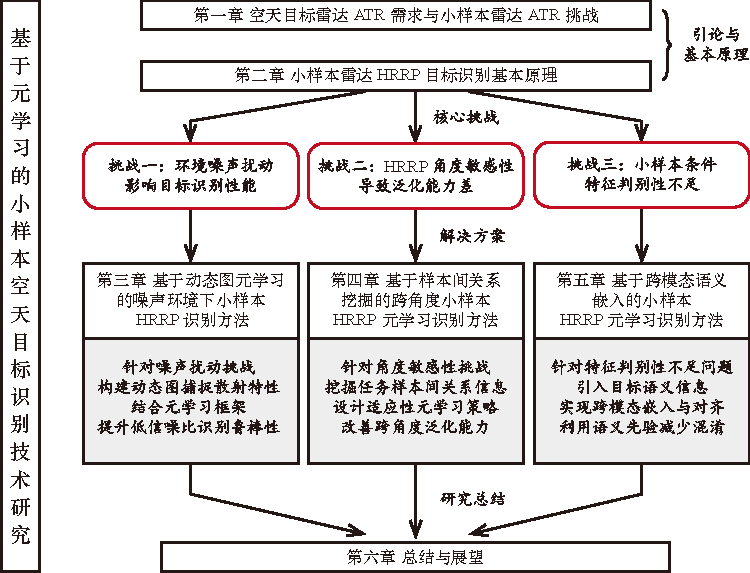
\includegraphics[width=0.95\linewidth]{figures/framework.pdf}
    \caption{本文组织架构和研究思路}
    \label{fig:framework}
\end{figure}

{第一章:绪论。} 作为开篇,本章首先阐明研究的宏观背景,即空天目标识别的重大国家战略需求;接着深入剖析RATR技术,包括其优势、固有局限以及当前发展趋势,并明确指出小样本问题是制约其发展的核心瓶颈;随后,对小样本RATR的研究现状、主要方法及面临的挑战进行综述,从而确立本论文的研究动机与定位;最后,概述本论文的主要研究工作和后续章节的内容安排。

{第二章:小样本雷达HRRP目标识别基本原理。} 本章为后续章节的研究提供必要的理论铺垫。内容包括:介绍宽带雷达成像与HRRP的基本原理、数学模型及其关键特性(如姿态敏感性);回顾基于深度学习的RATR框架;对小样本RATR问题进行形式化定义与分析,为后续提出基于元学习的解决方案奠定理论基础。

{第三章:基于动态图元学习的噪声环境下小样本HRRP识别方法。} 本章聚焦于第一个核心挑战:提升小样本HRRP识别的噪声鲁棒性。首先分析噪声对识别性能的影响机理。然后,详细阐述所提出的基于动态图元学习的识别方法,包括动态图构建策略、GNN表示学习模块、以及面向噪声鲁棒性的元学习框架设计与实现细节。最后,通过在含噪HRRP数据集上的仿真实验来验证方法的有效性,并与相关基线方法进行性能对比。

{第四章:基于样本间关系挖掘的跨角度小样本HRRP元学习识别方法。} 本章致力于解决第二个核心挑战:应对HRRP的角度敏感性。首先分析角度敏感性对小样本识别的制约。接着,详细介绍所提出的基于样本间关系挖掘的元学习方法,阐明如何利用图结构等机制建模样本间的角度关联,以及如何设计相应的元学习任务和优化策略来提升模型的角度泛化能力。最后,通过在具有角度变化的HRRP数据集上的实验,评估所提方法在跨角度小样本识别任务上的性能。

{第五章:基于跨模态语义嵌入的小样本HRRP元学习识别方法。} 本章旨在探索第三个核心方向:利用语义信息增强小样本HRRP识别。首先分析小样本下特征判别性不足的问题及引入语义的动机。然后,详细阐述融合跨模态语义嵌入的元学习方法,包括语义表示、HRRP特征提取(可能结合预训练模型)、跨模态融合机制、以及基于语义增强特征的元学习策略。最后,通过在含语义标签的HRRP数据集上的实验,验证该方法在提升小样本识别精度方面的效果。

{第六章:总结与展望。} 作为结尾,本章对全文的研究工作进行系统性总结,提炼主要的研究成果与创新点(即在利用元学习解决小样本HRRP识别的噪声鲁棒性、角度鲁棒性及语义融合问题上的贡献)。同时,客观地指出本研究存在的局限与待深入探讨的问题。最后,基于当前研究基础,对未来可能的研究方向进行展望。

	\chapter{小样本HRRP RATR 技术基本原理}
\label{chap:theory}

\section{引言}
\label{sec:theory_intro}

为了能够针对性地设计和改进元学习方法以适应小样本HRRP识别的特定需求,深刻理解其面临挑战的根源以及所能利用的理论工具至关重要。本章的核心任务正是为此奠定坚实的理论基础。我们将首先深入剖析HRRP的成像机理与数学表达,并着重分析其关键特性,尤其是导致识别困难的噪声影响和角度敏感性问题,为后续算法设计提供物理层面的洞察。接着,我们将回顾基于深度学习的RATR基本框架,明确元学习所依托或改进的现有模型基础。最后,也是本章的重点,我们将对小样本学习问题进行严格的形式化定义,并系统阐述元学习的基本概念、主流范式(基于优化、基于度量)及其核心算法机制,为后续章节中提出的创新元学习解决方案提供必要的算法背景和理论支撑。

本章具体内容安排如下:第\ref{sec:hrrp_mechanism}节介绍HRRP成像模型及特性分析;第\ref{sec:深度学习_ratr}节阐述基于深度学习的RATR技术框架与典型模型;第\ref{sec:fsl_modeling}节对小样本学习与元学习进行形式化定义并介绍基本框架;第\ref{sec:theory_summary}节对本章进行总结。

\section{空天目标宽带雷达成像机理}
\label{sec:hrrp_mechanism}

HRRP的形成是雷达系统发射宽带信号与目标发生电磁相互作用并经接收处理的结果。其精细结构蕴含了目标沿雷达视线(Line of Sight, LOS)方向的散射中心分布信息,是目标识别的重要依据。

\subsection{宽带雷达信号模型与HRRP成像}
\label{subsec:hrrp_imaging_model}

为了获得高的距离分辨率 $\Delta R$,现代雷达通常发射具有大带宽 $B$ 的信号。除了线性调频(Linear Frequency Modulated,LFM)信号,其他宽带信号形式如非线性调频、相位编码信号(如巴克码、P码)、频率步进信号等也可用于高分辨率成像,但LFM因其实现简单、易于产生大时宽带宽积而被广泛使用。一个典型的LFM发射信号 $s_t(t)$ 可以表示为:
\begin{equation}
    s_t(t) = \text{rect}\left(\frac{t}{T_p}\right) A_t \exp\left(j 2\pi f_c t + j \pi \gamma t^2\right)
    \label{eq:lfm_signal}
\end{equation}
其中,$t$ 表示快时间(Fast Time),$T_p$ 是脉冲持续时间,$A_t$ 是发射信号幅度,$f_c$ 是载波中心频率,$\gamma = B / T_p$ 是调频斜率。$\text{rect}(u)$ 是矩形窗函数。信号的瞬时频率为 $f(t) = f_c + \gamma t$,$t \in [-T_p/2, T_p/2]$,覆盖的带宽为 $B = |\gamma| T_p$。

假设目标可以由 $P$ 个理想的点散射中心模型近似描述。设第 $i$ 个散射中心的位置向量为 $\mathbf{r}_i$,其相对于雷达的初始距离为 $R_i = ||\mathbf{r}_i||$,对应的雷达散射系数为 $\sigma_i$(与频率、角度、极化相关)。在远场假设下,并考虑信号传播路径损耗,当雷达发射信号 $s_t(t)$ 后,经过目标散射并在雷达处接收到的回波信号 $s_r(t)$ 可以表示为所有散射中心回波的叠加:
\begin{equation}
    s_r(t) \approx \sum_{i=1}^{P} A_r \frac{\sigma_i}{R_i^2} s_t\left(t - \tau_i(t)\right)
    \label{eq:received_signal_sum_amplitude}
\end{equation}
其中,$A_r$ 是与雷达系统参数(如天线增益、发射功率)相关的幅度因子,$\tau_i(t) = 2 R_i(t) / c$ 是第 $i$ 个散射中心的瞬时双程传播时延,$R_i(t)$ 是 $t$ 时刻该散射中心到雷达的瞬时距离,$c$ 是光速。

在单个脉冲持续时间 $T_p$ 内,对于非机动或慢速目标,通常采用“冻结目标”或“走停”近似。在此近似下,$R_i(t) \approx R_i$。将回波信号下变频到基带,滤除高频项,并补偿固定的路径损耗和系统增益后,基带接收信号 $s_{r,base}(t)$ 近似为:
\begin{equation}
    s_{r,base}(t) \approx \sum_{i=1}^{P} \sigma'_i \text{rect}\left(\frac{t-\tau_i}{T_p}\right) \exp\left(j \pi \gamma (t-\tau_i)^2\right)
    \label{eq:received_baseband}
\end{equation}
其中 $\sigma'_i$ 是包含了幅度、散射相位以及传播相位 $\exp(-j 2\pi f_c \tau_i)$ 的等效复散射系数,$\tau_i = 2R_i/c$。

为了从接收信号中获得高距离分辨率,需要进行脉冲压缩处理,这通常通过与发射信号的复共轭进行匹配滤波来实现。匹配滤波器的冲激响应(基带形式)为 $h(t) = s_t^*(-t) \exp(-j 2\pi f_c t)$。匹配滤波器的输出 $s_o(t)$ 是输入信号与滤波器冲激响应的卷积:
\begin{equation}
    s_o(t) = s_{r,base}(t) * h(t) = \int_{-\infty}^{\infty} s_{r,base}(\tau) h(t-\tau) d\tau
    \label{eq:matched_filtering}
\end{equation}
对于理想的LFM信号和单个点目标,匹配滤波输出近似为一个峰值位于 $t = \tau_1$ 的sinc函数,其幅度包络为 $|\text{sinc}(B(t - \tau_1))|$。对于由多个散射中心组成的目标,在忽略散射中心之间的相互耦合以及满足分辨率要求的前提下,匹配滤波的输出近似为各个散射中心响应的相干叠加:
\begin{equation}
    s_o(t) \approx \sum_{i=1}^{P} \sigma''_i \text{sinc}\left(B(t - \tau_i)\right) \exp(-j 2\pi f_c \tau_i)
    \label{eq:pulse_compression_output_phase}
\end{equation}
其中 $\sigma''_i$ 是包含了原始散射幅度、脉冲压缩增益等因素的复幅度系数。此处的相位项 $\exp(-j 2\pi f_c \tau_i)$ 非常重要,它导致了不同散射中心响应之间的相干干涉。

HRRP通常定义为脉冲压缩后输出信号的幅度(或功率)沿距离轴的分布。令距离 $r = ct/2$,则HRRP函数 $p(r)$ 可以表示为:
\begin{equation}
    p(r) = |s_o(t)|_{t=2r/c} \approx \left| \sum_{i=1}^{P} \sigma''_i \text{sinc}\left(\frac{2B}{c}(r - R_i)\right) \exp(-j \frac{4\pi f_c R_i}{c}) \right|
    \label{eq:hrrp_definition_complex}
\end{equation}
其中 $R_i = c\tau_i/2$ 是第 $i$ 个散射中心沿雷达视线的投影距离。该式更清晰地表明,HRRP是目标各散射中心响应(具有幅度和相位)在距离轴上相干叠加后的幅度包络。其能够分辨两个散射中心的最小距离间隔,即距离分辨率 $\Delta R$,由信号带宽 $B$ 决定:
\begin{equation}
    \Delta R = \frac{\kappa c}{2B}
    \label{eq:range_resolution_kappa}
\end{equation}
其中 $\kappa$ 是与窗函数和分辨率定义相关的因子,对于矩形窗和瑞利准则(主瓣峰值到第一零点),$\kappa \approx 1$。实际应用中,为抑制旁瓣,常使用非矩形窗函数(如汉宁窗、海明窗),这会略微展宽主瓣,即 $\kappa > 1$。

然而,式~(\ref{eq:hrrp_definition_complex})描述的是理想情况下的HRRP。在实际雷达系统中,接收到的信号总是伴随着噪声和杂波。设 $n(t)$ 表示基带接收机噪声,通常建模为零均值加性高斯白噪声(Additive White Gaussian Noise, AWGN),其功率谱密度为 $N_0$。设 $c(t)$ 表示来自环境背景(地面、海面、云雨等)的杂波回波。则实际接收到的基带信号应为:
\begin{equation}
    s_{r,base}^{noisy}(t) = s_{r,base}(t) + c(t) + n(t)
    \label{eq:received_noisy}
\end{equation}
经过匹配滤波后,输出信号变为:
\begin{equation}
    s_o^{noisy}(t) = s_o(t) + c_o(t) + n_o(t)
    \label{eq:output_noisy}
\end{equation}
其中$s_o(t)$是理想目标回波的脉压输出,$c_o(t) = c(t) * h(t)$ 是杂波的脉压输出,$n_o(t) = n(t) * h(t)$ 是噪声的脉压输出。如果 $n(t)$ 是AWGN,则 $n_o(t)$ 也是零均值高斯过程,但不再是白噪声,其自相关函数由 $h(t)$ 决定。杂波 $c(t)$ 的统计特性通常更复杂,可能是非高斯的、相关的,并且其强度随距离、角度、环境类型(如不同地貌、海况)变化,常用的模型有瑞利分布(大量独立小散射体)、韦伯分布、对数正态分布或K分布(用于描述海杂波或地杂波的拖尾现象)\upcite{Jakeman1976806, Marier1995568, Ward1981561, Ozturk1995106}。

因此,实际观测到的HRRP样本 $p^{noisy}(r)$ 是含有噪声和杂波的脉压输出的幅度:
\begin{equation}
    p^{noisy}(r) = |s_o^{noisy}(t)|_{t=2r/c} = |s_o(t) + c_o(t) + n_o(t)|_{t=2r/c}
    \label{eq:hrrp_noisy}
\end{equation}
噪声和杂波的存在会污染甚至淹没目标信号 $s_o(t)$,导致HRRP形态失真、细节丢失、出现虚假峰值,从而严重影响识别性能。SNR或信杂比(Signal-to-Clutter Ratio, SCR)是衡量信号质量的重要指标。例如,脉压后的峰值信噪比可以定义为 $\text{SNR}_{peak} = \max |s_o(t)|^2 / E[|n_o(t)|^2]$。低SNR/SCR是RATR(特别是小样本RATR)面临的第一个严峻问题。虽然杂波(对应SCR)在特定环境(如地面、海面)下是主要的干扰源,其统计特性也更为复杂,但噪声(尤其是接收机热噪声,对应SNR)是雷达系统固有且普遍存在的干扰形式。AWGN模型因其数学上的易处理性和在算法性能评估中的基准地位,被广泛用于模拟和分析噪声对系统性能的影响。因此,本论文在后续章节研究算法的鲁棒性时,将主要聚焦于SNR条件下的性能,并主要采用AWGN模型来模拟噪声干扰,以此作为评估和提升算法在基础噪声环境下稳健性的关键途径,尽管对复杂杂波的抑制亦是重要的研究方向。 后续章节需要研究的算法应具备在低SNR下(即面对式~(\ref{eq:received_noisy})形式的输入时,其中噪声$n(t)$占主导地位)的鲁棒性。


现在我们来更形式化地描述HRRP的角度敏感性问题。如前所述,HRRP的形态依赖于目标姿态角 $(\theta, \phi)$。我们可以将理想HRRP函数显式地写为 $p(r; \theta, \phi)$,或者对于离散HRRP向量,记为 $\mathbf{p}(\theta, \phi) \in \mathbb{R}^N$。根据式~(\ref{eq:hrrp_definition_complex}),这种依赖性主要来源于投影距离 $R_i(\theta, \phi) = \mathbf{r}_i \cdot \hat{\mathbf{k}}(\theta, \phi)$ 和复幅度 $\sigma''_i(\theta, \phi)$ 对视线向量 $\hat{\mathbf{k}}(\theta, \phi)$ 的依赖。当姿态角发生一个微小的变化 $(\Delta\theta, \Delta\phi)$ 时,视线向量变化 $\Delta\hat{\mathbf{k}}$,导致投影距离变化 $\Delta R_i = \mathbf{r}_i \cdot \Delta\hat{\mathbf{k}}$,幅度 $\sigma''_i$ 也会发生变化 $\Delta\sigma''_i$。由于HRRP是相干叠加的结果,即使 $\Delta R_i$ 很小(小于 $\Delta R$),但其引起的相位变化 $\Delta\psi_i = - \frac{4\pi f_c}{c} \Delta R_i$ 可能很大(因 $f_c \gg B$),导致不同散射中心响应的干涉状态(相长或相消)发生剧烈改变,从而引起HRRP幅度 $p(r; \theta, \phi)$ 的快速振荡。我们可以用HRRP向量之间的距离(如欧氏距离)来衡量角度敏感性。对于同一目标 $y$,其在两个不同姿态角 $(\theta_1, \phi_1)$ 和 $(\theta_2, \phi_2)$ 下的HRRP样本 $\mathbf{p}_1 = \mathbf{p}(\theta_1, \phi_1)$ 和 $\mathbf{p}_2 = \mathbf{p}(\theta_2, \phi_2)$ 之间的距离 $d(\mathbf{p}_1, \mathbf{p}_2)$ 可能非常大,即使角度差 $\sqrt{(\theta_1-\theta_2)^2 + (\phi_1-\phi_2)^2}$ 很小。同时,可能存在另一个不同目标 $y'$ 在某个姿态角 $(\theta_3, \phi_3)$ 下的HRRP样本 $\mathbf{p}_3$ 与 $\mathbf{p}_1$ 非常接近,即 $d(\mathbf{p}_1, \mathbf{p}_3)$ 很小。这种现象即 $d(\mathbf{p}_1, \mathbf{p}_2) \gg d(\mathbf{p}_1, \mathbf{p}_3)$,其中 $y_1=y_2=y, y_3=y', y \neq y'$,严重违反了许多模式识别算法所依赖的“类内距离小、类间距离大”的假设。这就是HRRP角度敏感性对识别带来的核心困难,也是小样本RATR面临的第二个关键问题。后续章节需要设计的算法必须能够处理或减轻这种极端角度敏感性的影响。

\subsection{典型空天目标电磁散射特性}
\label{subsec:scattering_characteristics}

理解空天目标的电磁散射特性是深入分析HRRP数据并设计有效识别算法的基础。目标的散射特性决定了雷达接收到的回波信号的强度、相位、极化等信息,从而决定了HRRP的形态。

目标的雷达散射截面积(Radar Cross Section,RCS),记为 $\sigma$,是定量描述目标在特定方向上散射雷达波能力强弱的关键物理量。其严格定义为:
\begin{equation}
    \sigma = \lim_{R \to \infty} 4\pi R^2 \frac{P_s}{P_i} = \lim_{R \to \infty} 4\pi R^2 \frac{|\mathbf{E}_s|^2}{|\mathbf{E}_i|^2}
    \label{eq:rcs_definition}
\end{equation}
其中,$R$ 是距离,$P_i$ 和 $P_s$ 分别是入射和散射功率密度,$\mathbf{E}_i$ 和 $\mathbf{E}_s$ 分别是入射和散射电场强度。RCS具有面积的量纲,单位通常是平方米(m²)或分贝平方米(dBsm)。对于一个复杂目标,RCS不仅依赖于目标的物理属性(尺寸、形状、材料),还强烈地依赖于雷达的工作参数(频率 $f_c$、极化方式 $\text{pol}$)和观测几何(入射波方向 $(\theta_i, \phi_i)$ 和散射波方向 $(\theta_s, \phi_s)$)。对于单站雷达,入射和散射方向相同,RCS通常表示为 $\sigma(f_c, \text{pol}, \theta, \phi)$,其中 $(\theta, \phi)$ 是目标本体坐标系下的姿态角。

根据电磁场理论,在高频区(目标尺寸远大于波长 $\lambda = c/f_c$),目标的总散射场可以看作是由目标表面感应电流和感应磁流辐射产生的场,其贡献主要来自于局部区域,可以分解为几种基本的散射机制\upcite{Pathak199244, Song19971488, KELLER1962116, Ling1989194, Kouyoumjian19741448}。镜面反射发生在尺寸远大于波长的光滑曲面上,满足几何光学反射定律,散射能量集中在镜面反射方向,通常形成RCS方向图中的强峰值。边缘绕射发生在目标几何形状的突变处,如机翼、尾翼的边缘,舵面、舱门的缝隙边缘等。根据几何绕射理论(Geometrical Theory of Diffraction,GTD),边缘绕射的能量相对较弱,但方向性比镜面反射弱,可在更宽的角度范围内观测到\upcite{kohama_gtd_2011}。尖顶或角点绕射发生在目标的尖顶(如机头、导弹弹头)或角点处。爬行波是电磁波入射到目标光滑曲面的阴影边界时,激发沿表面传播的波,并在目标的背向区域再次辐射,对低频散射和阴影区散射有重要贡献。行波是在细长结构(如机翼前缘、天线臂)上,入射波可能激发沿结构传播的波,并在端点或不连续处产生辐射。腔体散射对于具有开放式腔体结构的目标(如飞机的发动机进气道、尾喷口,座舱等)非常重要,入射电磁波会进入腔体内部,经过多次反射和模式转换后再辐射出来,可能形成非常强的散射,并且其散射特性对频率和观测角度通常极为敏感\upcite{anastassiu_review_2003}。一个复杂空天目标(如飞机)的RCS随姿态角的变化曲线通常呈现出极其复杂的起伏形态,峰谷差异可达数十dB,并且在很小的角度间隔内就可能发生剧烈变化\upcite{xu_rcs_1991}。这是因为随着姿态角的改变,雷达视线照射到目标的不同部位,主导的散射机制会发生转换,同时来自不同散射中心的贡献之间的相干干涉关系也会随之改变,导致总散射场的强度发生快速振荡。

为了在高频区对目标的散射特性进行建模和分析,散射中心模型被广泛应用\upcite{liu_scnet_2024, Gerry19991179, Potter19951058, KELLER1962116, Hurst1987986}。该模型将目标的总散射场近似为来自目标上有限个离散的等效散射中心的贡献的相干叠加。属性散射中心模型(Attributed Scattering Center Model,ASCM)是其中一种常用模型\upcite{Potter199779},它不仅给出了散射中心的位置,还描述了其散射强度随频率和角度变化的特性。根据ASCM,第 $i$ 个散射中心对总散射场 $E_s$ 的贡献 $E_i$ 可以表示为频率 $f$ 和视线向量 $\hat{\mathbf{k}}$ 的函数:
\begin{equation}
    E_i(f, \hat{\mathbf{k}}) \approx A_i(\text{pol}) \left(\frac{j f}{f_{ref}}\right)^{\alpha_i} \mathcal{S}_i(f, \hat{\mathbf{k}}) \exp\left(-j \frac{4\pi f}{c} \mathbf{r}_i \cdot \hat{\mathbf{k}}\right)
    \label{eq:ascm}
\end{equation}
在此式中,$A_i(\text{pol})$ 是第 $i$ 个散射中心在参考频率 $f_{ref}$ 和特定极化下的复幅度。$\alpha_i$ 是频率依赖因子,描述了散射幅度随频率的变化关系,其取值与散射机制类型有关(例如,$\alpha_i=1$ 对应镜面反射,$\alpha_i=0$ 对应边缘绕射)。$\mathcal{S}_i(f, \hat{\mathbf{k}})$ 是角度依赖因子,描述散射强度随观测角度的变化。对于局部化散射中心,$\mathcal{S}_i \approx 1$;对于分布式散射中心(如长直边缘),$\mathcal{S}_i$ 可能具有 $\text{sinc}$ 函数形式。$\mathbf{r}_i$ 是第 $i$ 个散射中心的位置向量。$\exp(-j \frac{4\pi f}{c} \mathbf{r}_i \cdot \hat{\mathbf{k}})$ 是由位置决定的相位项,其中 $\mathbf{r}_i \cdot \hat{\mathbf{k}} = R_i$ 即为该散射中心沿视线的投影距离。将式~(\ref{eq:ascm})代入宽带回波模型并进行脉冲压缩,即可得到基于散射中心模型的HRRP表达式。可以看出,HRRP的形态直接由各散射中心的位置 $\mathbf{r}_i$、类型 $\alpha_i$、强度 $A_i$ 以及它们随频率 $f$ 和视线 $\hat{\mathbf{k}}$ 的变化规律 $\mathcal{S}_i$ 共同决定。当姿态角 $(\theta, \phi)$ 变化时,$\hat{\mathbf{k}}$ 改变,导致相位项中的投影距离 $R_i$、角度依赖因子 $\mathcal{S}_i$ 以及可能的幅度 $A_i$ 都发生变化,进而造成HRRP形态的剧烈改变。这进一步从物理模型层面印证了HRRP的角度敏感性。

需要指出的是,除了HRRP所反映的目标沿雷达视线的静态散射结构信息外,目标的部件级运动(即微动),例如飞机涡轮发动机叶片的旋转、直升机旋翼的转动、导弹弹体的进动或章动等,也会在雷达回波中引入除主体平动多普勒之外的附加频率调制,产生微多普勒效应\upcite{gurbuz_data-driven_2018}。这些微多普勒特征蕴含了关于目标内部结构和运行状态的独特动态信息,是目标识别的另一类重要信息来源,尤其对于区分外形相似但内部运动部件不同的目标具有关键作用。然而,微多普勒特征的提取与分析通常依赖于时频分析技术\upcite{yu_local_2019, huang_parameterized_2021, chithra_comprehensive_2023},这与本研究关注的、主要基于脉冲压缩后HRRP幅度信息的识别方法在信号处理层面和特征维度上均有显著不同。鉴于本论文聚焦于解决小样本条件下HRRP识别所面临的噪声鲁棒性与角度敏感性等核心挑战,对微多普勒特征的深入研究与利用将不作为本文探讨的重点,后续章节将集中讨论基于HRRP本身及其衍生特征的识别方法。

综上所述,空天目标复杂的几何结构和材料构成导致了其独特的电磁散射特性,这种特性对频率和观测角度高度敏感,是形成复杂多变HRRP数据的物理根源。深刻理解这些散射机理和特性,对于后续章节中设计能够适应HRRP数据复杂性(特别是角度敏感性)和环境干扰(如噪声)的鲁棒识别算法至关重要。

\section{基于深度学习的RATR技术}
\label{sec:深度学习_ratr}

近年来,深度学习凭借其强大的特征学习和非线性建模能力,已成为推动RATR技术发展的主要动力。基于深度学习的RATR方法旨在通过构建深度神经网络模型,自动从雷达数据中学习具有判别力的特征表示,实现端到端的识别。

\subsection{RATR 的深度学习框架}
\label{subsec:深度学习_framework}

基于深度学习的RATR系统通常遵循一个标准的监督学习框架。假设拥有训练数据集 $D_{train} = \{(\mathbf{x}_i, y_i)\}_{i=1}^{M}$,其中 $\mathbf{x}_i \in \mathcal{X}$ 是雷达观测数据(如HRRP向量 $\mathbf{p}_i \in \mathbb{R}^N$),$y_i \in \mathcal{Y} = \{1, \dots, C\}$ 是对应的目标类别标签。目标是学习一个映射函数 $f_\Theta: \mathcal{X} \rightarrow \mathcal{Y}$,该函数由参数 $\Theta$ 控制,能对未知样本 $\mathbf{x}$ 预测其类别 $\hat{y} = f_\Theta(\mathbf{x})$。

在深度学习框架下,$f_\Theta$ 通常由一个深度神经网络(Deep Neural Network,DNN)实现,可视为复合函数,由多个层组成,每层对其输入进行线性变换和非线性激活。一个包含 $L$ 层的前馈神经网络可表示为:
\begin{align}
    \mathbf{a}^{(l)} &= W^{(l)} \mathbf{h}^{(l-1)} + \mathbf{b}^{(l)} \label{eq:dnn_linear} \\
    \mathbf{h}^{(l)} &= \sigma^{(l)}(\mathbf{a}^{(l)}) \label{eq:dnn_activation}
\end{align}
其中,$l=1, \dots, L$ 是层索引,$\mathbf{h}^{(l)} \in \mathbb{R}^{d_l}$ 是第 $l$ 层的输出,$\mathbf{h}^{(0)} = \mathbf{x}$ 是输入。$W^{(l)} \in \mathbb{R}^{d_l \times d_{l-1}}$ 和 $\mathbf{b}^{(l)} \in \mathbb{R}^{d_l}$ 是权重和偏置。$\sigma^{(l)}(\cdot)$ 是非线性激活函数(如ReLU)。整个网络的参数为 $\Theta = \{W^{(l)}, \mathbf{b}^{(l)}\}_{l=1}^{L}$。

对于 $C$ 类分类任务,最后一层输出 $C$ 维的 logits $\mathbf{z} = \mathbf{a}^{(L)}$。通过 Softmax 函数将 logits 转换为概率分布 $\mathbf{p}(\mathbf{x}) = [p(y=1|\mathbf{x}), \dots, p(y=C|\mathbf{x})]^T$:
\begin{equation}
    p(y=c|\mathbf{x}; \Theta) = \frac{\exp(z_c)}{\sum_{c'=1}^{C} \exp(z_{c'})}, \quad c=1, \dots, C
    \label{eq:softmax}
\end{equation}
最终预测标签 $\hat{y}$ 选择概率最高的类别:
\begin{equation}
    \hat{y} = f_\Theta(\mathbf{x}) = \arg\max_{c \in \{1, \dots, C\}} p(y=c|\mathbf{x}; \Theta)
    \label{eq:prediction}
\end{equation}

模型训练的目标是找到最优参数 $\Theta^*$,使模型在训练数据 $D_{train}$ 上的预测尽可能准确,并具有良好的泛化能力。这通过最小化损失函数 $\mathcal{L}$ 实现。常用的是交叉熵损失:
\begin{equation}
    \mathcal{L}_{CE}(f_\Theta(\mathbf{x}_i), y_i) = -\sum_{c=1}^{C} \mathbb{I}(y_i=c) \log p(y=c|\mathbf{x}_i; \Theta) = -\log p(y=y_i|\mathbf{x}_i; \Theta)
    \label{eq:cross_entropy_loss}
\end{equation}
其中 $\mathbb{I}(\cdot)$ 是指示函数。训练目标是最小化训练集上的平均损失,通常加入正则化项 $\Omega(\Theta)$ 防止过拟合:
\begin{equation}
    \Theta^* = \arg\min_{\Theta} \left\{ \frac{1}{M} \sum_{i=1}^{M} \mathcal{L}_{CE}(f_\Theta(\mathbf{x}_i), y_i) + \lambda \Omega(\Theta) \right\}
    \label{eq:optimization_objective}
\end{equation}
其中 $\lambda \ge 0$ 是正则化系数。此优化问题通常采用基于梯度的迭代算法求解,如随机梯度下降(Stochastic Gradient Descent,SGD)及其变种\upcite{Bottou2018223, LeCun19982278}。利用反向传播算法计算梯度 $\nabla_\Theta \mathcal{L}$,并更新参数:
\begin{equation}
    \Theta_{t+1} \leftarrow \Theta_t - \eta_t \nabla_\Theta \mathcal{L}(\Theta_t; D_{batch})
    \label{eq:sgd_update}
\end{equation}
其中 $\eta_t$ 是学习率。

% --- 示意图占位符 ---
\begin{figure}[h!]
    \centering
    % \includegraphics[width=0.9\linewidth]{figures/深度学习_framework.pdf}
    \fbox{图 2.1: 基于深度学习的RATR框架示意图 (占位符)}
    \caption{基于深度学习的RATR框架示意图}
    \label{fig:深度学习_framework}
\end{figure}

\subsection{典型深度学习模型及其适用性}
\label{subsec:typical_深度学习_models}

立足于前述基于深度学习的RATR通用框架,针对HRRP数据独特的物理属性与表征形式,研究界已发展并应用了多种特定的深度神经网络架构。HRRP作为目标一维散射信息的载体,其数据形态呈现为一维序列 $\mathbf{p} \in \mathbb{R}^N$($N$为距离单元数),蕴含着丰富的局部结构信息(如散射中心的位置、强度、形状),同时也表现出对观测角度和噪声的高度敏感性。这些特性共同决定了并非所有深度学习模型都同样适用于HRRP识别任务,模型的选择与设计必须充分考虑如何有效提取HRRP中的判别性信息,同时抑制敏感性带来的负面影响。因此,研究人员已成功探索并适配了包括CNN、RNN、LSTM、Transformer以及自编码器(Atuo-Encoder,AE)等多种深度模型,它们各自凭借不同的结构优势,在HRRP特征学习与识别任务中展现出独特的适用性与潜力。

一维卷积神经网络(1D-CNN)因其在提取局部空间(或时间)模式方面的强大能力,并具有一定的平移不变性,被广泛应用于处理HRRP这类一维序列数据\upcite{song_radar_2019, guo_radar_2019}。对于输入HRRP向量 $\mathbf{p} \in \mathbb{R}^{N \times C_{in}}$(这里假设输入可以有 $C_{in}$ 个通道,例如原始幅度、相位或不同预处理结果;若仅为幅度,则 $C_{in}=1$),一个1D-CNN层包含 $C_{out}$ 个卷积核(Filter)。第 $j$ ($j=1, \dots, C_{out}$) 个卷积核 $\mathbf{K}_j \in \mathbb{R}^{F \times C_{in}}$($F$ 为核尺寸)在输入序列上以步长 $S$ 滑动,并考虑填充 $P$(Padding)。输出特征图 $\mathbf{H}_j \in \mathbb{R}^{N'}$ 的第 $n$ 个元素通过以下卷积操作计算得到:
\begin{equation}
    H_{j,n} = \sigma\left( \sum_{c=1}^{C_{in}} \sum_{f=1}^{F} K_{j,f,c} \, p_{n \cdot S + f - P', c} + b_j \right)
    \label{eq:1d_cnn_conv_detailed}
\end{equation}
其中,$p_{n',c}$ 是输入序列在位置 $n'$、通道 $c$ 的值(经过填充处理),$K_{j,f,c}$ 是第 $j$ 个核在位置 $f$、输入通道 $c$ 的权重,$b_j$ 是第 $j$ 个核对应的偏置,$P'$ 与填充 $P$ 和核中心有关,$\sigma(\cdot)$ 是非线性激活函数(如ReLU, LeakyReLU)。输出特征图的长度 $N' = \lfloor (N + 2P - F) / S \rfloor + 1$。通过堆叠多个卷积层(使用不同的核尺寸、步长、填充和通道数,或引入空洞卷积以增大感受野而不增加参数),模型能够学习到HRRP中从低级的边缘、纹理模式到高级的散射中心组合结构的层次化特征表示。

在卷积层之间或之后,通常会插入池化层(Pooling Layer),如最大池化(Max Pooling)或平均池化(Average Pooling)。池化操作在一个局部窗口(大小为 $F_p$,步长为 $\mathcal{S}_p$)内对特征图进行下采样。例如,最大池化输出为:
\begin{equation}
    H'_{j,n} = \max_{i=(n-1)\mathcal{S}_p+1}^{\min(n\mathcal{S}_p, N')} H_{j,i}
    \label{eq:max_pooling}
\end{equation}
池化层的主要作用是降低特征图的空间维度(长度),减少计算量和参数数量,并提供一定程度的局部平移不变性,增强模型对HRRP轻微平移或形变的鲁棒性。

为了构建更深、更有效的CNN模型,研究者引入了先进的网络结构。残差网络 (Residual Network,ResNet)\upcite{resnet} 通过引入“跳跃连接”(Skip Connection)来缓解深度网络训练中的梯度消失问题。其核心思想是学习残差映射 $\mathcal{F}(\mathbf{h}^{(l-1)})$,并将输入 $\mathbf{h}^{(l-1)}$ 直接加到输出上:
\begin{equation}
    \mathbf{h}^{(l)} = \sigma(\mathcal{F}(\mathbf{h}^{(l-1)}; \mathbf{W}^{(l)}) + \mathbf{h}^{(l-1)})
    \label{eq:resnet_block}
\end{equation}
这种恒等映射的捷径使得梯度能够更容易地反向传播到浅层。密集连接网络 (Densely Connected Convolutional Network,DenseNet)\upcite{huang_2017_cvpr} 则更进一步,将每一层与其后所有层直接连接,每一层的输入包含了前面所有层的特征图的拼接:
\begin{equation}
    \mathbf{h}^{(l)} = \sigma(\mathbf{W}^{(l)} [\mathbf{h}^{(0)}, \mathbf{h}^{(1)}, \dots, \mathbf{h}^{(l-1)}] + \mathbf{b}^{(l)})
    \label{eq:densenet_block}
\end{equation}
其中 $[\cdot]$ 表示特征图在通道维度上的拼接。DenseNet通过最大化信息流和特征重用,可以用更少的参数达到很高的性能。这些结构都可以适配到1D-CNN中,用于构建更强大的HRRP特征提取器。1D-CNN因其对局部结构信息的强大捕捉能力,特别适合提取HRRP中由散射中心及其相对位置关系所决定的特征。

RNN及其变种特别适合处理具有时序或序列依赖性的数据。当HRRP数据以随时间 $t$ 或角度 $\alpha$ 变化的序列 $\mathbf{P} = (\mathbf{p}_1, \mathbf{p}_2, \dots, \mathbf{p}_T)$ 形式给出时($\mathbf{p}_t \in \mathbb{R}^N$),RNN能够通过其内部的循环结构来建模序列中的动态信息。标准的RNN在时刻 $t$ 计算隐藏状态 $\mathbf{h}_t \in \mathbb{R}^{d_h}$,该状态依赖于当前输入 $\mathbf{p}_t \in \mathbb{R}^N$ 和前一时刻的隐藏状态 $\mathbf{h}_{t-1}$:
\begin{equation}
    \mathbf{h}_t = \sigma_h(\mathbf{W}_{hh} \mathbf{h}_{t-1} + \mathbf{W}_{xh} \mathbf{p}_t + \mathbf{b}_h)
    \label{eq:rnn_recurrence_dim}
\end{equation}
其中 $\mathbf{W}_{hh} \in \mathbb{R}^{d_h \times d_h}$ 和 $\mathbf{W}_{xh} \in \mathbb{R}^{d_h \times N}$ 是权重矩阵,$\mathbf{b}_h$ 是偏置,$\sigma_h$ 是激活函数。隐藏状态 $\mathbf{h}_t$ 理论上编码了从序列开始到时刻 $t$ 的所有信息。最终的序列表示(如 $\mathbf{h}_T$ 或所有隐藏状态的某种聚合)被用于分类。然而,标准RNN在处理长序列时会遇到梯度消失或爆炸的问题,难以学习长距离依赖关系\upcite{pan_radar_2022}。

LSTM\upcite{tu_novel_2019, jithesh_lstm_2017}通过引入精巧的门控机制(遗忘门 $\mathbf{f}_t$、输入门 $\mathbf{i}_t$、输出门 $\mathbf{o}_t$)和一个独立的细胞状态 $\mathbf{C}_t \in \mathbb{R}^{d_h}$ 来克服这一问题。这些门控制着信息的流入、流出以及在细胞状态中的长期保存。其更新过程如下(输入为 $[\mathbf{h}_{t-1}, \mathbf{p}_t] \in \mathbb{R}^{d_h+N}$):
\begin{align}
    \mathbf{f}_t &= \sigma_g(\mathbf{W}_f [\mathbf{h}_{t-1}, \mathbf{p}_t] + \mathbf{b}_f) \in \mathbb{R}^{d_h} \label{eq:lstm_f_dim} \\
    \mathbf{i}_t &= \sigma_g(\mathbf{W}_i [\mathbf{h}_{t-1}, \mathbf{p}_t] + \mathbf{b}_i) \in \mathbb{R}^{d_h} \label{eq:lstm_i_dim} \\
    \tilde{\mathbf{C}}_t &= \sigma_c(\mathbf{W}_C [\mathbf{h}_{t-1}, \mathbf{p}_t] + \mathbf{b}_C) \in \mathbb{R}^{d_h} \label{eq:lstm_c_tilde_dim} \\
    \mathbf{C}_t &= \mathbf{f}_t \odot \mathbf{C}_{t-1} + \mathbf{i}_t \odot \tilde{\mathbf{C}}_t \in \mathbb{R}^{d_h} \label{eq:lstm_c_dim} \\
    \mathbf{o}_t &= \sigma_g(\mathbf{W}_o [\mathbf{h}_{t-1}, \mathbf{p}_t] + \mathbf{b}_o) \in \mathbb{R}^{d_h} \label{eq:lstm_o_dim} \\
    \mathbf{h}_t &= \mathbf{o}_t \odot \sigma_h(\mathbf{C}_t) \in \mathbb{R}^{d_h} \label{eq:lstm_h_dim}
\end{align}
其中 $\mathbf{W}_f, \mathbf{W}_i, \mathbf{W}_C, \mathbf{W}_o \in \mathbb{R}^{d_h \times (d_h+N)}$ 是权重矩阵,$\odot$ 是逐元素乘积,$\sigma_g$ 通常是Sigmoid,$\sigma_c, \sigma_h$ 通常是Tanh。LSTM能够更有效地学习和记忆长序列中的依赖关系。门控循环单元(Gated Recurrent Unit, GRU)是LSTM的一个简化变种。双向RNN、LSTM (BiRNN、BiLSTM) 则通过同时处理正向和反向序列,能够捕捉每个时刻的过去和未来上下文信息,其输出 $\mathbf{h}_t = [\overrightarrow{\mathbf{h}}_t; \overleftarrow{\mathbf{h}}_t]$。卷积LSTM (ConvLSTM) 则将卷积操作引入LSTM的门计算中,适合处理时空序列数据。这些RNN及其变种非常适合建模HRRP随角度变化的动态特性,或者捕捉单个HRRP内部沿距离单元的顺序依赖关系\upcite{zeng_radar_2022, pan_radar_2022, tu_novel_2019, jithesh_lstm_2017, yang_radar_2024}。

注意力机制\upcite{pan_radar_2022} 可以与RNN、LSTM等序列模型结合,使模型能够动态地、有选择地关注输入序列(或隐藏状态序列)中与当前任务最相关的部分。例如,在序列到序列模型中,解码器在生成每个输出时,会计算一个注意力权重分布 $\boldsymbol{\alpha}_t$ 在编码器所有时刻隐藏状态 $\{\mathbf{h}_i^{enc}\}$ 上,然后计算一个上下文向量 $\mathbf{c}_t = \sum_i \alpha_{ti} \mathbf{h}_i^{enc}$,该向量包含了当前最相关的源序列信息,并被用于辅助解码。注意力机制提高了模型处理长序列和对齐输入输出的能力。

近年来,完全基于自注意力机制(Self-Attention)的Transformer模型\upcite{vaswani_attention_2017, li_mtbc_2025, gao_polarimetric_2024, yang_radar_2024} 在序列处理任务上取得了巨大成功,并开始被探索用于HRRP识别。其核心是自注意力层,它计算序列中每个元素(例如HRRP序列中的一个样本,或单个HRRP中的一个距离单元表示)与其他所有元素之间的相关性权重,并据此聚合信息来更新自身表示。标准的缩放点积注意力计算如下:
\begin{equation}
    \text{Attention}(\mathbf{Q}, \mathbf{K}, \mathbf{V}) = \text{softmax}\left(\frac{\mathbf{Q}\mathbf{K}^T}{\sqrt{d_k}}\right)\mathbf{V}
    \label{eq:scaled_dot_product_attention}
\end{equation}
其中 $\mathbf{Q}, \mathbf{K}, \mathbf{V}$ 分别是由输入序列通过线性变换得到的查询、键、值矩阵。Transformer通常采用多头注意力(Multi-Head Attention),即并行地计算多个独立的注意力头,然后将结果拼接并再次线性变换,以捕捉不同子空间中的不同依赖关系:
\begin{equation}
    \text{MultiHead}(\mathbf{Q}, \mathbf{K}, \mathbf{V}) = \text{Concat}(\text{head}_1, \dots, \text{head}_H) \mathbf{W}^O
    \label{eq:multi_head_attention}
\end{equation}
其中 $\text{head}_h = \text{Attention}(\mathbf{Q}\mathbf{W}_h^Q, \mathbf{K}\mathbf{W}_h^K, \mathbf{V}\mathbf{W}_h^V)$。Transformer通过堆叠自注意力层和前馈网络层,能够并行地捕捉序列内任意两个位置之间的长距离依赖关系,这对于理解HRRP序列的角度演化或HRRP内部散射中心的复杂相互作用可能具有优势。

AE及其变种是一类重要的无监督学习模型,旨在学习数据的有效压缩表示(编码)并能从中重构原始数据(解码)。基础AE由编码器 $g_\phi: \mathcal{X} \rightarrow \mathcal{Z}$ 和解码器 $f_\psi: \mathcal{Z} \rightarrow \mathcal{X}$ 组成,$\mathcal{Z}$ 是通常维度较低的隐空间 $\mathbb{R}^{d_z}$ ($d_z \ll \text{dim}(\mathcal{X})$)。它们通常由多层神经网络实现,例如:
\begin{align}
    \mathbf{z} &= g_\phi(\mathbf{x}) = \sigma_e(\mathbf{W}_e^{(L_e)} \dots \sigma_e(\mathbf{W}_e^{(1)} \mathbf{x} + \mathbf{b}_e^{(1)}) \dots + \mathbf{b}_e^{(L_e)}) \label{eq:ae_encoder_mlp} \\
    \hat{\mathbf{x}} &= f_\psi(\mathbf{z}) = \sigma_d(\mathbf{W}_d^{(L_d)} \dots \sigma_d(\mathbf{W}_d^{(1)} \mathbf{z} + \mathbf{b}_d^{(1)}) \dots + \mathbf{b}_d^{(L_d)}) \label{eq:ae_decoder_mlp}
\end{align}
训练目标是最小化输入 $\mathbf{x}$ 与重构输出 $\hat{\mathbf{x}}$ 之间的重构误差,如均方误差 (MSE):
\begin{equation}
    \phi^*, \psi^* = \arg\min_{\phi, \psi} \mathbb{E}_{\mathbf{x} \sim p_{data}(\mathbf{x})} [ ||\mathbf{x} - f_\psi(g_\phi(\mathbf{x}))||^2 ]
    \label{eq:ae_objective_mse}
\end{equation}
训练完成后,编码器 $g_{\phi^*}$ 可以提取输入数据的低维、非线性特征表示 $\mathbf{z}$,用于后续的分类、降维等任务。

AE有多种重要变种:稀疏自编码器(Sparse AE)\upcite{guo_method_2020} 通过在损失函数中加入对隐层激活值的稀疏性惩罚(如L1正则项或KL散度),迫使模型学习到更具信息量和可解释性的稀疏表示。去噪自编码器 (Denoising AE, DAE)\upcite{wu_cae_2023, Vincent2008DAE} 的输入是原始数据 $\mathbf{x}$ 的一个损坏版本 $\tilde{\mathbf{x}}$(例如加入高斯噪声),而目标是重构出干净的原始数据 $\mathbf{x}$。其优化目标为:
\begin{equation}
    \phi^*, \psi^* = \arg\min_{\phi, \psi} \mathbb{E}_{(\mathbf{x}, \tilde{\mathbf{x}})} [ ||\mathbf{x} - f_\psi(g_\phi(\tilde{\mathbf{x}}))||^2 ]
    \label{eq:dae_objective}
\end{equation}
通过强制模型从噪声中恢复信号,DAE能够学习到对输入扰动更鲁棒的特征表示,非常适合用于HRRP信号的去噪和鲁棒特征提取。变分自编码器(Variational AE, VAE)\upcite{zhai_robust_2017, Kingma2014VAE} 则是一种生成模型,它假设隐变量 $\mathbf{z}$ 服从某个先验分布 $p(\mathbf{z})$(通常是标准正态分布),并学习一个概率编码器 $q_\phi(\mathbf{z}|\mathbf{x})$(输出 $\mathbf{z}$ 的均值 $\boldsymbol{\mu}_\phi(\mathbf{x})$ 和方差 $\boldsymbol{\sigma}^2_\phi(\mathbf{x})$)和一个概率解码器 $p_\psi(\mathbf{x}|\mathbf{z})$。其优化目标(证据下界,ELBO)包含重构项和正则化项(编码器后验与先验的KL散度):
\begin{equation}
    \mathcal{L}_{VAE} = \mathbb{E}_{q_\phi(\mathbf{z}|\mathbf{x})}[-\log p_\psi(\mathbf{x}|\mathbf{z})] - D_{KL}(q_\phi(\mathbf{z}|\mathbf{x}) || p(\mathbf{z}))
    \label{eq:vae_objective}
\end{equation}
VAE不仅能学习特征表示,还能通过从先验分布 $p(\mathbf{z})$ 中采样并送入解码器 $p_\psi(\mathbf{x}|\mathbf{z})$ 来生成新的HRRP样本,在数据增广方面有应用潜力\upcite{zhang_patch-wise_2023}。

这些深度学习模型为HRRP RATR提供了强大的表示学习能力。然而,它们的成功通常依赖于大量的、覆盖目标各种状态的标注数据。当数据量严重不足时(即小样本场景),这些参数量巨大的模型极易过拟合,泛化能力差,这正是FSL和元学习需要解决的核心问题。
\section{小样本RATR问题建模}
\label{sec:fsl_modeling}

FSL旨在使机器学习模型能够像人类一样,从极少数的样本中学习识别新的概念。元学习是实现FSL的一种主流且有效的范式,其核心思想是“学会学习”。本节将对FSL问题进行形式化定义,介绍元学习框架,并结合HRRP特性阐述小样本条件下特征判别性不足和语义信息利用匮乏问题的形式化理解。

\subsection{小样本学习定义}
\label{subsec:fsl_definition}

FSL问题通常设定在一个与监督学习不同的场景中。假设存在两个类别集合:基类别 $C_{base}$ 和新类别 $C_{novel}$,它们之间没有交集,即 $C_{base} \cap C_{novel} = \emptyset$。我们拥有一个基础数据集 $D_{base} = \{(\mathbf{x}_i, y_i) | y_i \in C_{base}\}_{i=1}^{M_{base}}$,其中包含来自基类别的大量标注样本。目标是利用在 $D_{base}$ 上学习到的知识,使模型能够在面对来自新类别 $C_{novel}$ 的任务时表现良好,即使每个新类别 $c \in C_{novel}$ 只有极少数($K$个)标注样本可用。这种设定被称为 $K$-shot 学习,其中 $K$ 通常很小(如1或5)。同时,任务通常涉及从 $C_{novel}$ 中区分 $N$ 个类别,称为 $N$-way $K$-shot 问题。

为了有效地训练和评估能够解决FSL问题的模型,研究界广泛采用了基于任务的训练范式(S/Q Training)\upcite{li_libfewshot_2023, achille_task2vec_2019, achille_task2vec_2019, achille_task2vec_2019, maurer_benefit_2016}。该范式通过在训练阶段模拟测试时的小样本场景来进行。具体来说,训练过程不是在整个 $D_{base}$ 上一次性完成,而是通过从 $D_{base}$ 中反复采样生成大量模拟的小样本学习任务。一个典型的 $N$-way $K$-shot 分类任务 $\mathcal{T}$ 的构建过程如下:首先,从 $C_{base}$ 中随机无放回地选择 $N$ 个类别,构成该任务的类别子集 $C_{\mathcal{T}}$。然后,对于 $C_{\mathcal{T}}$ 中的每一个类别 $c$,从 $D_{base}$ 中该类别的样本里随机选择 $K$ 个标注样本,构成该任务的支持集(Support Set) $\mathcal{S}_{\mathcal{T}} = \{(\mathbf{x}_i^s, y_i^s)\}_{i=1}^{N \times K}$,其中 $y_i^s \in C_{\mathcal{T}}$。支持集的作用是提供给模型在该特定任务上进行学习或适应的少量信息。接着,对于这 $N$ 个类别 $C_{\mathcal{T}}$,再从 $D_{base}$ 中(确保与 $\mathcal{S}_{\mathcal{T}}$ 中的样本不同)选择一批样本,构成该任务的查询集(Query Set) $\mathcal{Q}_{\mathcal{T}} = \{(\mathbf{x}_j^q, y_j^q)\}_{j=1}^{N_q}$,其中 $y_j^q \in C_{\mathcal{T}}$。查询集用于评估模型在利用支持集 $\mathcal{S}_{\mathcal{T}}$ 进行学习/适应后的性能。通常,每个类别的查询样本数量 $N_q/N$ 会大于 $K$。

模型的训练目标是在大量按某种分布 $p(\mathcal{T})$ 采样生成的任务 $\mathcal{T}$ 上进行优化,使其能够最小化在各个任务查询集上的期望损失。通过这种在大量不同的小样本任务上进行“演练”的训练方式,期望模型能够学习到一种通用的、跨任务的“元知识”或“学习策略”。拥有这种能力的模型,在元测试(Meta-Testing)阶段,当面对一个由来自新类别 $C_{novel}$ 构成的、同样是 $N$-way $K$-shot 设置的新任务 $\mathcal{T}_{novel}$ 时,就能够利用其支持集 $\mathcal{S}_{novel}$ 快速适应,并对其查询集 $\mathcal{Q}_{novel}$ 中的样本做出准确的预测\upcite{tripuraneni_provable_2021, du_few-shot_2020}。

在小样本HRRP RATR问题中,$\mathbf{x}$ 是HRRP样本(向量 $\mathbf{p}$ 或序列 $\mathbf{P}$),$y$ 是目标类别标签。$D_{base}$ 可能是包含若干常见目标类型(如飞机A、B、C)在多种姿态角、多种信噪比下的大量HRRP样本。$C_{novel}$ 则包含一些新的、稀有的目标类型(如飞机X、Y、Z),每种只有 $K$ 个标注样本。训练时模拟大量 $N$-way $K$-shot 任务,测试时则在由 $C_{novel}$ 构成的 $N$-way $K$-shot 任务上评估模型的泛化识别能力。

小样本学习的核心困难在于,当每个类别的样本数量 $K$ 极小时,标准监督学习训练的深度模型 $f_\Theta$ 往往无法学习到具有良好泛化性的特征表示。这尤其体现在特征判别性不足的问题上。理想情况下,模型学习到的特征提取器 $\phi_\theta$(例如DNN的倒数第二层输出)应将来自同一类别的样本(即使它们由于姿态、噪声等原因看起来差异很大)映射到特征空间中的紧凑区域,并将不同类别的区域分离开。然而,当 $K$ 很小时,模型从每个类别看到的样本非常有限,可能无法捕捉到该类别的本质、不变的特征,而更容易关注到样本特有的、偶然的细节或噪声。这导致学习到的嵌入空间中,同类样本可能分散得很开(类内差异大),而不同类别的样本(特别是物理特征相似的类别)可能相互混杂(类间距离小)。形式化地,假设 $\phi_\theta(\mathbf{x})$ 是样本 $\mathbf{x}$ 的嵌入向量,对于属于类别 $y$ 的样本,其类内散布矩阵 $\mathcal{S}_W = \sum_{c=1}^C \sum_{\mathbf{x}: y=c} (\phi_\theta(\mathbf{x}) - \mu_c)(\phi_\theta(\mathbf{x}) - \mu_c)^T$($\mu_c$ 为类别 $c$ 的均值向量)的迹可能很大,而类间散布矩阵 $\mathcal{S}_B = \sum_{c=1}^C N_c (\mu_c - \mu)(\mu_c - \mu)^T$($\mu$ 为总均值, $N_c$ 为类别 $c$ 样本数)的迹相对较小,导致 Fisher 判别准则 $J = \text{tr}(\mathcal{S}_W^{-1} \mathcal{S}_B)$ 很小,即可分性差。这是小样本RATR面临的第三个关键问题(特征判别性不足)的数学根源之一。

此外,标准的模型 $f_\Theta(\mathbf{x})$ 通常只接收物理观测数据 $\mathbf{x}$ 作为输入。然而,如第一章所述,目标的语义信息 $s$(如功能类别、型号家族等)在小样本或特征模糊时可能提供重要的补充判别线索。当前框架下,语义信息 $s$ 并未被利用,即模型是 $f_\Theta(\mathbf{x})$ 而非 $f_\Theta(\mathbf{x}, s)$。这种语义信息利用的匮乏,形式上表现为模型输入空间的局限性,是小样本RATR面临的第三个问题的另一方面。后续章节将探讨如何将语义信息 $s$ 有效地融入学习框架。

\subsection{基于元学习的小样本 RATR 框架}
\label{subsec:meta_learning_framework}

元学习为解决上述FSL问题提供了一个强大的理论框架,旨在通过在大量相关任务上的学习,让模型掌握一种能够快速适应新任务的通用学习能力或先验知识(元知识)。形式化地,元学习的目标是学习一个元学习器 $\mathcal{A}$,其自身可能包含一组元参数 $\Phi$。当给定新任务 $\mathcal{T}$ 的支持集 $\mathcal{S}_{\mathcal{T}}$ 时,元学习器能利用 $\mathcal{S}_{\mathcal{T}}$ 适应自身,对查询样本 $\mathbf{x}^q$ 做出预测 $\hat{y}^q = \mathcal{A}(\mathbf{x}^q | \mathcal{S}_{\mathcal{T}}; \Phi)$。元训练过程(Meta-Training)旨在找到最优元参数 $\Phi^*$,使得元学习器在任务分布 $p(\mathcal{T})$ 上的期望性能最优。这通常通过最小化在所有训练任务 $\mathcal{T}_i \sim p(\mathcal{T})$ 上的平均损失来实现:
\begin{equation}
    \Phi^* = \arg\min_{\Phi} \mathbb{E}_{\mathcal{T}_i=(\mathcal{S}_i, \mathcal{Q}_i) \sim p(\mathcal{T})} [\mathcal{L}_{\mathcal{T}_i}(\Phi)]
    \label{eq:meta_objective}
\end{equation}
其中,$\mathcal{L}_{\mathcal{T}_i}(\Phi)$ 是元学习器在任务 $\mathcal{T}_i$ 上的损失,通常定义为在给定支持集 $\mathcal{S}_i$ 条件下,在查询集 $\mathcal{Q}_i$ 上的平均损失:
\begin{equation}
    \mathcal{L}_{\mathcal{T}_i}(\Phi) = \frac{1}{N_q} \sum_{j=1}^{N_q} \mathcal{L}( \mathcal{A}(\mathbf{x}_j^q | \mathcal{S}_i; \Phi), y_j^q )
    \label{eq:task_loss_meta}
\end{equation}
$\mathcal{L}(\cdot, \cdot)$ 是基学习任务的损失函数(如交叉熵)。元参数 $\Phi$ 的优化通常也采用基于梯度的优化方法。以下介绍两种主流的元学习范式:

基于度量学习的元学习方法,其核心是学习一个通用的嵌入函数 $\phi_\theta: \mathcal{X} \rightarrow \mathbb{R}^d$(参数 $\theta$ 即元参数 $\Phi$),将HRRP样本映射到嵌入空间,使得同类样本靠近,异类样本远离。对于新任务 $\mathcal{T}=(S, Q)$,识别过程为:计算支持集 $S$ 中每个类别 $n$ 的原型 $\mathbf{c}_n$(通常是该类支持样本嵌入向量的均值):
\begin{equation}
    \mathbf{c}_n = \frac{1}{K} \sum_{\{(\mathbf{x}_i^s, y_i^s) \in S \mid y_i^s=n\}} \phi_\theta(\mathbf{x}_i^s)
    \label{eq:prototype_calculation}
\end{equation}
然后将查询样本 $\mathbf{x}^q$ 映射为 $\phi_\theta(\mathbf{x}^q)$,并根据其与各原型 $\mathbf{c}_n$ 的距离 $d(\cdot, \cdot)$(如欧氏距离平方)进行分类,例如选择距离最近的原型对应的类别:
\begin{equation}
    \hat{y}^q = \arg\min_{n \in \{1, \dots, N\}} d(\phi_\theta(\mathbf{x}^q), \mathbf{c}_n)
    \label{eq:protonet_prediction_argmin}
\end{equation}
或者通过Softmax计算概率:
\begin{equation}
    p(y=n | \mathbf{x}^q, S; \theta) = \frac{\exp(-\gamma d(\phi_\theta(\mathbf{x}^q), \mathbf{c}_n))}{\sum_{n'=1}^{N} \exp(-\gamma d(\phi_\theta(\mathbf{x}^q), \mathbf{c}_{n'}))}
    \label{eq:protonet_prediction_softmax_gamma} % Added gamma
\end{equation}
其中 $\gamma$ 是尺度参数。在元训练阶段,参数 $\theta$ 通过最小化在大量采样任务查询集上的负对数似然损失来学习:
\begin{equation}
    \theta^* = \arg\min_{\theta} \mathbb{E}_{\mathcal{T}_i \sim p(\mathcal{T})} \left[ \sum_{(\mathbf{x}_j^q, y_j^q) \in \mathcal{Q}_i} -\log p(y=y_j^q | \mathbf{x}_j^q, \mathcal{S}_i; \theta) \right]
    \label{eq:protonet_meta_objective}
\end{equation}
ProtoNet\upcite{snell_prototypical_2017, tian_open_2022}是这类方法的典型代表。其他基于度量的方法还包括MN\upcite{vinyals_matching_2016}(使用注意力机制计算查询与支持样本的相似度)和RelationNet\upcite{sung_relation_2018}(使用一个神经网络来学习相似度度量)。这类方法的优点是简洁、高效。然而,标准的度量学习方法可能对噪声敏感(噪声影响嵌入向量和距离计算),并且难以处理HRRP的极端角度敏感性(同一目标不同角度样本在嵌入空间可能距离很远,破坏原型代表性)。后续章节将针对这些问题对基于度量学习的元学习框架进行改进。

% --- 示意图占位符 ---
\begin{figure}[h]
    \centering
    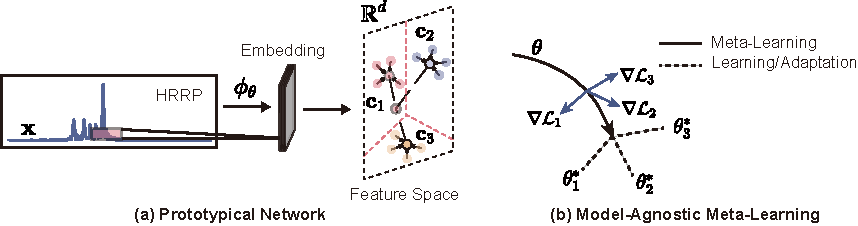
\includegraphics[width=\linewidth]{figures/proto_maml.pdf}
    % \fbox{图 2.2: ProtoNet工作原理示意图 (占位符)}
    \caption{典型元学习方法ProtoNet、MAML工作原理示意图}
    \label{fig:protonet}
\end{figure}

基于优化的元学习方法,其目标是学习一个模型的初始参数 $\theta_0$(作为元参数 $\Phi$),使得该初始参数能通过在新任务 $\mathcal{T}_i$ 的支持集 $\mathcal{S}_i$ 上进行少量梯度下降更新,快速适应到对该任务最优的参数 $\theta_i'$。MAML\upcite{finn_model-agnostic_2017}是该方向的代表作。其元训练包含两个嵌套优化循环。内循环是任务适应:对于任务 $\mathcal{T}_i=(\mathcal{S}_i, \mathcal{Q}_i)$,从当前元参数 $\theta$ 出发,使用 $\mathcal{S}_i$ 计算损失 $\mathcal{L}_{\mathcal{S}_i}(\theta)$,并进行一步或 $U$ 步梯度下降更新得到任务特定参数 $\theta_i'$。例如,一步更新:
\begin{equation}
    \theta_i'(\theta) = \theta - \alpha \nabla_\theta \mathcal{L}_{\mathcal{S}_i}(\theta)
    \label{eq:maml_inner_update}
\end{equation}
其中 $\alpha$ 是内循环学习率。外循环是元优化:使用 $\mathcal{Q}_i$ 评估适应后的模型 $f_{\theta_i'}$,计算损失 $\mathcal{L}_{\mathcal{Q}_i}(\theta_i')$。元参数 $\theta$ 的更新基于所有任务的查询集损失梯度:
\begin{equation}
    \theta \leftarrow \theta - \beta \nabla_\theta \left( \sum_{\mathcal{T}_i \sim p(\mathcal{T})} \mathcal{L}_{\mathcal{Q}_i}(\theta_i'(\theta)) \right)
    \label{eq:maml_outer_update}
\end{equation}
其中 $\beta$ 是外循环学习率。计算元梯度 $\nabla_\theta \mathcal{L}_{\mathcal{Q}_i}(\theta_i'(\theta))$ 通常需要二阶导数,计算成本较高,存在一阶近似方法如FOMAML\upcite{yang_few-shot_2022}和Reptile\upcite{nichol_reptile_2018}以及简化方法ANIL\upcite{aniruddh_anil_2020}。MAML的核心是找到一个对任务损失变化敏感的初始化点。其优点是模型无关性。然而,MAML的训练可能不稳定,且对于HRRP的角度敏感性问题,仅仅几步梯度更新是否足以适应剧烈的特征变化也是一个疑问。

% --- 示意图占位符 ---
% \begin{figure}[h!]
%     \centering
%     \includegraphics[width=0.4\linewidth]{figures/maml.pdf}
%     % \fbox{图 2.3: MAML工作原理示意图 (占位符)}
%     \caption{MAML工作原理示意图}
%     \label{fig:maml}
% \end{figure}

元学习框架为解决小样本RATR问题提供了强大武器。通过元训练,模型有望学习到关于HRRP数据、类别关系及学习策略的元知识,从而在面对真实小样本场景时表现出更好的泛化性和适应能力。后续章节将深入探讨如何将元学习框架与针对性机制结合,以应对噪声、角度敏感性及语义信息利用不足等具体问题。

\section{本章小结}
\label{sec:theory_summary}
本章首先从物理层面深入剖析了HRRP的成像机理,推导了宽带雷达信号模型与HRRP的数学表达式,揭示了其与目标散射中心分布的关系及距离分辨率特性。通过引入噪声与杂波模型,形式化了低SNR对HRRP识别构成的第一个关键问题。进一步地,结合电磁散射理论和散射中心模型分析,阐明了HRRP对姿态角 $p(r; \theta, \phi)$ 的极端敏感性源于散射投影变化和相干干涉,并指出这是识别面临的第二个关键问题。这些分析为后续章节理解HRRP数据特性、应对噪声干扰与角度变化奠定了物理基础。

其次,本章回顾了基于深度学习的RATR框架,包括优化目标和典型模型。接着,对FSL问题进行了形式化定义,引入了S/Q Training范式,并从特征空间角度分析了小样本下特征判别性不足及语义信息 $s$ 缺失构成的第三个关键问题。最后,重点介绍了元学习框架及基于度量学习和基于优化这两大主流范式的数学原理。本章通过梳理相关基础理论并形式化关键问题,为后续章节针对性地提出基于元学习的解决方案提供了统一的数学语言和坚实的理论铺垫。
	
	
%%% Local Variables:
%%% mode: latex
%%% TeX-master: "../main"
%%% End:

\begin{ack}
报考国防科大,始于少年时的荧屏记忆。哈军工前辈的身影,学者风骨,军人本色,在那个年代交织辉映。曾向往那样的场景:与战友并肩奔跑,也探讨着科学;灯下捧着饭盒,仍调试着仪器。那是心之所向。如今在科大,昔日憧憬已是日常,前行的脚步也因此更加踏实。

深深感谢国防科技大学这片沃土。常想,若非在此经历“两个转变”的心志淬炼,我难有今日这份笃定。是科大,推着我一步步走出舒适区,去迎接那些曾经的畏惧:从克服内心障碍、站上英语演讲台获得认可,到连续两年带队远赴巴黎、在国际赛场上历练,终获大型赛事奖项十余项。这些昔日未敢奢望的突破,都源于科大提供的平台与机遇。这片独特的熔炉,锻造了勇气,也见证了成长。

在此,谨向我的导师户盼鹤副教授致以最深的敬意与感谢。读研路上,户老师是引路人,亦是同行者。他将宝贵的经验倾囊相授,以恳切的教诲照亮前路。多少个夜晚,无论多晚,他总把学生的事放在心上,耐心解答我的每一个疑问。从课题方向的把握到技术细节的斟酌,户老师总是与我平等交流,细致探讨,既有学者的严谨,亦有师长的温和。他常教导我们,要有纯正的学术追求,要从部队的实际出发,去解决真问题。这份言传身教,如春风化雨,将伴我一生。

感谢我的招生老师游鹏老师。您是我初入科大的领路人。正是您的关心与指导,让我得以更快地融入这里的学习与生活节奏,开始认识并实现自我价值。

感谢教研室的黎湘老师、刘永祥老师、姜卫东老师、高勋章老师、刘振老师、刘丽老师、张双辉老师、刘天鹏老师、张文鹏老师、杨威老师、沈亲沐老师、卢哲俊老师、夏靖远老师、苏晓龙老师、智帅峰老师、张新禹老师、李俊老师、刘烁伟老师、李铭洋老师、林煌星老师、张志远老师和李瑞泽老师。感谢您们为我的课题严格把关,提出的宝贵意见如同路标,指引方向。亦感谢您们在日常中给予的关心与帮助。感谢办公室助理张煌、钟仪、颜学钦、王肖、高柯,感谢硬件工程师苏建伟、杨近松、朱乾坤。感谢你们的默默付出与支持,让我得以更加心无旁骛地投入到学习与研究之中。

感谢刘旗师兄、邱祥风师兄、程耘师兄、姜辣师兄、潘之梁师兄、郭金兴师兄、廖淮璋师兄、杨志雄师兄、李伟杰师兄、周洁师姐、刘阿飞师兄、张家伟师兄、易拓源师兄、卞小贝师姐、张青青师姐、王朋朋师兄、孙潇师兄、陈冠潮师兄、孙浩彬师兄、王泽昊师兄、张振家师兄、程晨师兄、涂晓未师兄。与你们的交流,常能激荡出思想的火花。无论学业难题还是生活点滴,你们总能凭借过来人的经验,给予我中肯而温暖的建议。这种亦师亦友的情谊,弥足珍贵。

感谢湖南省科学技术厅的经费支持。主持湖南省自然科学基金青年学生基础研究项目的这段经历,不仅是科研能力的集中锻炼,更是对独立承担责任、系统推进工作的宝贵实践。这段经历为我未来的科研道路奠定了坚实基础,其益无穷。

感谢理学院生化系Zhu's Lab、计算机学院天河生物医药团队、前沿交叉学院光电所、军政基础教育学院军事外语系、理学院数学系我的指导老师们,你们是我科研生涯的启蒙者。在全球、全国顶级赛事四年的锻炼,极大拓展了我的学科视野,夯实了我的科研基本功,赋予了我独立承担课题、勇于探索创新的底气。

感谢电子科学学院一大队一队全体人员,感谢大家四年的陪伴。感谢贺海军、高兴亮、黄源、叶俊、杨亚洲、辛熙鹤、李威、徐佳、邹斐帆队长和教导员们,你们是我军旅人生的灯塔,没有你们搭的“梯子”,我也无法吃上“盘子”。感谢同级的范文刚、徐丞柏、黄意扬、韩天放、刘洋、奚齐、周骜、徐浚熙、杨颖、黄昕睿、陆嘉杰、范昊、冯世宇、杨姿等战友,我们同甘共苦,希望你们未来越来越好!

最后,感谢我的家人。你们默默的理解与无条件的支持,是我能够安心求学、勇往直前的最坚实后盾和最温暖港湾。

行文至此,思绪万千,谨以此四言小诗作结,聊表寸心:

\begin{center}
负笈湘皋,问道穷源。\\
格物致知,淬砺心坚。\\
家国之任,未敢等闲。\\
来日骋志,更谱新篇。\\
鹏程初展,好风正悬。\\
前路修远,步履弥坚。\\
感念师友,德谊绵长。\\
丹心如铁,辉映朝阳。
\end{center}

\vspace{2\baselineskip} % 增加一些垂直间距
\begin{flushright}
{\kaishu 陈凌峰~~~~~~~~~~~} \\ % 请替换为您的姓名
2025年5月于长沙 % 请替换为实际年月
\end{flushright}
  
\end{ack}

	
	\cleardoublepage
	\phantomsection
	\addcontentsline{toc}{chapter}{参考文献}
	\bibliographystyle{bstutf8}
	\bibliography{ref/refs}
	
	\begin{resume}
   %评阅版论文隐去阶段性成果具体信息,保留此段文字:
	
  %该论文作者在学期间取得的阶段性成果(学术论文等)已满足我校博士学位评 阅相关要求。为避免阶段性成果信息对专家评价学位论文本身造成干扰,特将论文作者的阶段性成果信息隐去。
  
  \section*{1. 学术论文} % 发表的和录用的合在一起

  \begin{enumerate}[label={[\arabic*]},itemsep=0pt,parsep=0pt,labelindent=26pt,labelwidth=*,leftmargin=0pt,itemindent=*,align=left]
   %[label=\textbf{[\arabic*]},itemindent=*, align=left] %老版本缩进对齐
   
  %\addtolength{\itemsep}{-.36\baselineskip}%缩小条目之间的间距,下面类似
  \item \textbf{\underline{Chen L}}, Sun X, Pan Z, Wang Z, Su X, Liu Z and Hu P. Make HRRPs to Be Graphs for Efficient Target Recognition [J]. IET Electronics Letters, 2024, 60(22):e70088. (SCI已发表,影响因子:1.202,一作.)
  \item \textbf{\underline{Chen L}}, Hu P, Pan Z, Sun X and Wang Z. A Deep Learning-Based Target Radial Length Estimation Method through HRRP Sequence [C]. 2024 IEEE 12th Asia-Pacific Conference on Antennas and Propagation (APCAP 2024), 2024. (EI已发表,一作.)
  \item \textbf{\underline{Chen L}}, Hu P, Pan Z, Sun X, Wang Z. Advancing Few-shot HRRP Target Recognition with Meta-learning and Graph Neural Network [C]. 中国电子学会第一届空天信息技术大会(AITC 2024), 2024.(获评“空天之星”优秀报告,一作.)
  \item Fan H, \textbf{\underline{Chen L}}, Xu C, Zhou J, Dai Y and Hu P. Few-shot Human Motion Recognition through Multi-Aspect mmWave FMCW Radar Data [C]. 2025 IEEE 45th International Symposium on Geoscience and Remote Sensing (IGARSS 2025), 2025. (CCF-C/EI已录用,二作兼通讯.)
  \item Feng S, \textbf{\underline{Chen L}}, Su X, Liu Q and Hu P. Enhancing HRRP RATR Robustness to Incomplete Aspect Angles via Supervised Contrastive Learning [C]. 2025 IEEE 10th International Conference on Intelligent Computing and Signal Processing (ICSP 2025), 2025. (EI已录用,二作.)
  \item 潘之梁,户盼鹤,\textbf{\underline{陈凌峰}},刘振. 基于深度增强IST网络的ISAR稀疏成像 [J]. 海军航空大学学报, 2024, 39(5):603-614. (中文核心.)
  \item Pan Z, Hu P, \textbf{\underline{Chen L}}, Su X and Liu Z. An ISAR Cross-range Scaling Method Based on Track Information [C]. 2024 IEEE 14th International Conference on Microwave and Millimeter Wave Technology (ICMMT 2024), 2024.(EI已录用.)
  \item \textbf{\underline{Chen L}}, Pan Z, Liu Q and Hu P. HRRPGraphNet++: Dynamic Graph Neural Network with Meta-Learning for Few-shot HRRP Radar Target Recognition [J]. MDPI Remote Sensing. (SCI在审,一作.)
  \item \textbf{\underline{Chen L}}, Hu Pan, Liu Q and Liu Z. GAF-MLGNN: An Efficient Meta-Learning Framework for Few-shot HRRP RATR with GNN. IEEE Transactions on Signal and Information Processing over Networks [J], 2025. (SCI在审,一作.)
  \item \textbf{\underline{Chen L}}, Hu P and Liu Z. Seeing What Few-shot Learners See: Contrastive Cross-Class Attribution for Explainability [C]. (CCF-A/EI在审,一作.)
  \item Hu P, \textbf{\underline{Chen L}}, Zhang Z and Liu Z. Feature Fusion CGAN Based HRRP Denoising and Reconstruction Method [J]. Chinese Journal of Electronics, 2025. (SCI在审,大修意见,通讯.)
  \end{enumerate}

  \section*{2. 发明专利} % 有就写,没有就删除
  \begin{enumerate}[label={[\arabic*]},itemsep=0pt,parsep=0pt,labelindent=26pt,labelwidth=*,leftmargin=0pt,itemindent=*,align=left]
  %[label=\textbf{[\arabic*]},itemindent=*, align=left] %老版本缩进对齐
  %\addtolength{\itemsep}{-.36\baselineskip}%
  \item 户盼鹤,\textbf{\underline{陈凌峰}},潘之梁,苏晓龙,王泽昊,刘振. 基于HRRP序列的目标径向长度估计方法、装置、设备和介质:ZL202411235169.5 (专利号.)
  \item 
  \item 
  \item 
  \item 
  \item 一种基于深度展开IAA网络的频谱估计方法.
  \item 户盼鹤,\textbf{\underline{陈凌峰}},潘之梁,苏晓龙,王泽昊,刘振. 基于深度学习的HRRP 序列目标径向长度估计方法及装置:202411251160.3 (申请号.)
  \end{enumerate}

    \section*{3. 科研项目} % 有就写,没有就删除
  \begin{enumerate}[label={[\arabic*]},itemsep=0pt,parsep=0pt,labelindent=26pt,labelwidth=*,leftmargin=0pt,itemindent=*,align=left]
  %[label=\textbf{[\arabic*]},itemindent=*, align=left] %老版本缩进对齐
  %\addtolength{\itemsep}{-.36\baselineskip}%
  \item 
  \end{enumerate}
\end{resume}

	% 最后,需要的话还要生成附录,全文随之结束。
	\appendix
	\backmatter
	% TeX
\chapter{模板提供的希腊字母命令列表}

大写希腊字母:
\begin{table}[htbp]
\centering
\begin{tabular}{llll}
\toprule
$\Gamma$~\verb|\Gamma| & $\Lambda$~\verb|\Lambda| & $\Sigma$~\verb|\Sigma| & $\Psi$~\verb|\Psi| \\
$\Delta$~\verb|\Delta| & $\Xi$~\verb|\Xi| & $\Upsilon$~\verb|\Upsilon| & $\Omega$~\verb|\Omega| \\
$\Theta$~\verb|\Theta| & $\Pi$~\verb|\Pi| & $\Phi$~\verb|\Phi| & \\
\midrule
$\varGamma$~\verb|\varGamma| & $\varLambda$~\verb|\varLambda| & $\varSigma$~\verb|\varSigma| & $\varPsi$~\verb|\varPsi| \\
$\varDelta$~\verb|\varDelta| & $\varXi$~\verb|\varXi| & $\varUpsilon$~\verb|\varUpsilon| & $\varOmega$~\verb|\varOmega| \\
$\varTheta$~\verb|\varTheta| & $\varPi$~\verb|\varPi| & $\varPhi$~\verb|\varPhi| & \\
\bottomrule
\end{tabular}
\end{table}

小写希腊字母:
\begin{table}[htbp]
\centering
\begin{tabular}{llll}
\toprule
$\alpha$~\verb|\alpha| & $\theta$~\verb|\theta| & $o$~\verb|o| & $\tau$~\verb|\tau| \\ 
$\beta$~\verb|\beta| & $\vartheta$~\verb|\vartheta| & $\pi$~\verb|\pi| & $\upsilon$~\verb|\upsilon| \\ 
$\gamma$~\verb|\gamma| & $\iota$~\verb|\iota| & $\varpi$~\verb|\varpi| & $\phi$~\verb|\phi| \\ 
$\delta$~\verb|\delta| & $\kappa$~\verb|\kappa| & $\rho$~\verb|\rho| & $\varphi$~\verb|\varphi| \\ 
$\epsilon$~\verb|\epsilon| & $\lambda$~\verb|\lambda| & $\varrho$~\verb|\varrho| & $\chi$~\verb|\chi| \\ 
$\varepsilon$~\verb|\varepsilon| & $\mu$~\verb|\mu| & $\sigma$~\verb|\sigma| & $\psi$~\verb|\psi| \\ 
$\zeta$~\verb|\zeta| & $\nu$~\verb|\nu| & $\varsigma$~\verb|\varsigma| & $\omega$~\verb|\omega| \\ 
$\eta$~\verb|\eta| & $\xi$~\verb|\xi| & $\varkappa$~\verb|\varkappa| & $\digamma$~\verb|\digamma| \\ 
\midrule
$\upalpha$~\verb|\upalpha| & $\uptheta$~\verb|\uptheta| & $\mathrm{o}$~\verb|\mathrm{o}| & $\uptau$~\verb|\uptau| \\ 
$\upbeta$~\verb|\upbeta| & $\upvartheta$~\verb|\upvartheta| & $\uppi$~\verb|\uppi| & $\upupsilon$~\verb|\upupsilon| \\ 
$\upgamma$~\verb|\upgamma| & $\upiota$~\verb|\upiota| & $\upvarpi$~\verb|\upvarpi| & $\upphi$~\verb|\upphi| \\ 
$\updelta$~\verb|\updelta| & $\upkappa$~\verb|\upkappa| & $\uprho$~\verb|\uprho| & $\upvarphi$~\verb|\upvarphi| \\ 
$\upepsilon$~\verb|\upepsilon| & $\uplambda$~\verb|\uplambda| & $\upvarrho$~\verb|\upvarrho| & $\upchi$~\verb|\upchi| \\ 
$\upvarepsilon$~\verb|\upvarepsilon| & $\upmu$~\verb|\upmu| & $\upsigma$~\verb|\upsigma| & $\uppsi$~\verb|\uppsi| \\ 
$\upzeta$~\verb|\upzeta| & $\upnu$~\verb|\upnu| & $\upvarsigma$~\verb|\upvarsigma| & $\upomega$~\verb|\upomega| \\ 
$\upeta$~\verb|\upeta| & $\upxi$~\verb|\upxi| & & \\ 
\bottomrule
\end{tabular}
\end{table}

希腊字母属于数学符号类别,请用\verb|\bm|命令加粗,其余向量、矩阵可用\verb|\mathbf|。

	
\end{document}
